\section{Feature Extraction and Analysis}
\label{sec:sae}

The critical notions introduced in Section~\ref{sec:foundations}, together with the hypotheses about the structure of neural network representations discussed in Section~\ref{sec:hypotheses}, provide the conceptual foundation for developing methods to identify and analyse manipulable internal objects associated with concepts of interest, i.e., features. One straightforward paradigm is to decompose model activations into sparse linear features. Sparse autoencoders (SAEs) provide a principled example of this approach, learning to represent any input activation with a subset of a large dictionary of monosemantic, interpretable features~\citeest{cunningham2023sparse}.

This section first introduces the canonical sparse coding problem and links it to SAEs, reviews how SAEs extract interpretable features, and then provides a practical overview and comparison of major SAE variants. We then introduce methods for multi-layer feature extraction and analysis, such as transcoders and crosscoders, and compare them with SAEs as well as with a broader range of alternative feature-extraction methods.

\subsection{The Sparse Coding Problem}
Early neuroscience studies posited that brains represent information using sparse, interpretable basis signals~\citeest{Barlow:1961aa, sparsecoding}. This hypothesis further motivated research to decompose natural images and compare the decomposed signals with cell activities in the primary visual cortex, finding surprising alignment~\citeest{olshausen1996emergence, olshausen1997sparse}. At the same time, the signal processing community has also examined representing a given signal as the sum of a subset of basis signals from a given overcomplete dictionary~\citeest{matchingpursuit, basispursuit}. Studies on learning better overcomplete dictionaries for high-quality representations also thrived~\citeest{lewicki2000learning, aharon2006k}. Together, they framed the sparse dictionary learning research question, with SAEs serving as a modern algorithm that uses neural network activations as the signal. Specifically, given data $h$, a sparse dictionary learning method finds the dictionary $D$ and sparse codes $z$ such that
\begin{equation}
h \approx Dz \text{ and } \|z\|_0 \text{ is small}.
\end{equation}
SAEs implement this with neural networks: $h$ are model activations, $D = W_{\text{out}}$ is an overcomplete dictionary to learn, and the sparse codes are $z = \sigma(W_{\text{in}} h + b_{\text{in}})$. Note that conventional dictionary methods usually run the algorithm to find a $z$ for each $h$, which does not scale to modern language models. In contrast, SAEs use a nonlinear encoder $E$ to predict the coefficients for different input activations.

\subsection{Sparse Autoencoders}
\label{subsec:sae-foundation}

SAEs (Figure~\ref{fig:sae}) extract monosemantic features from polysemantic model activations. They are trained to reconstruct activations at a specific location in neural networks, such as the output of an MLP block or an entire transformer layer (i.e., the residual stream), while keeping only a few features active in any given forward pass.

\begin{figure}[tb]
  \centering
    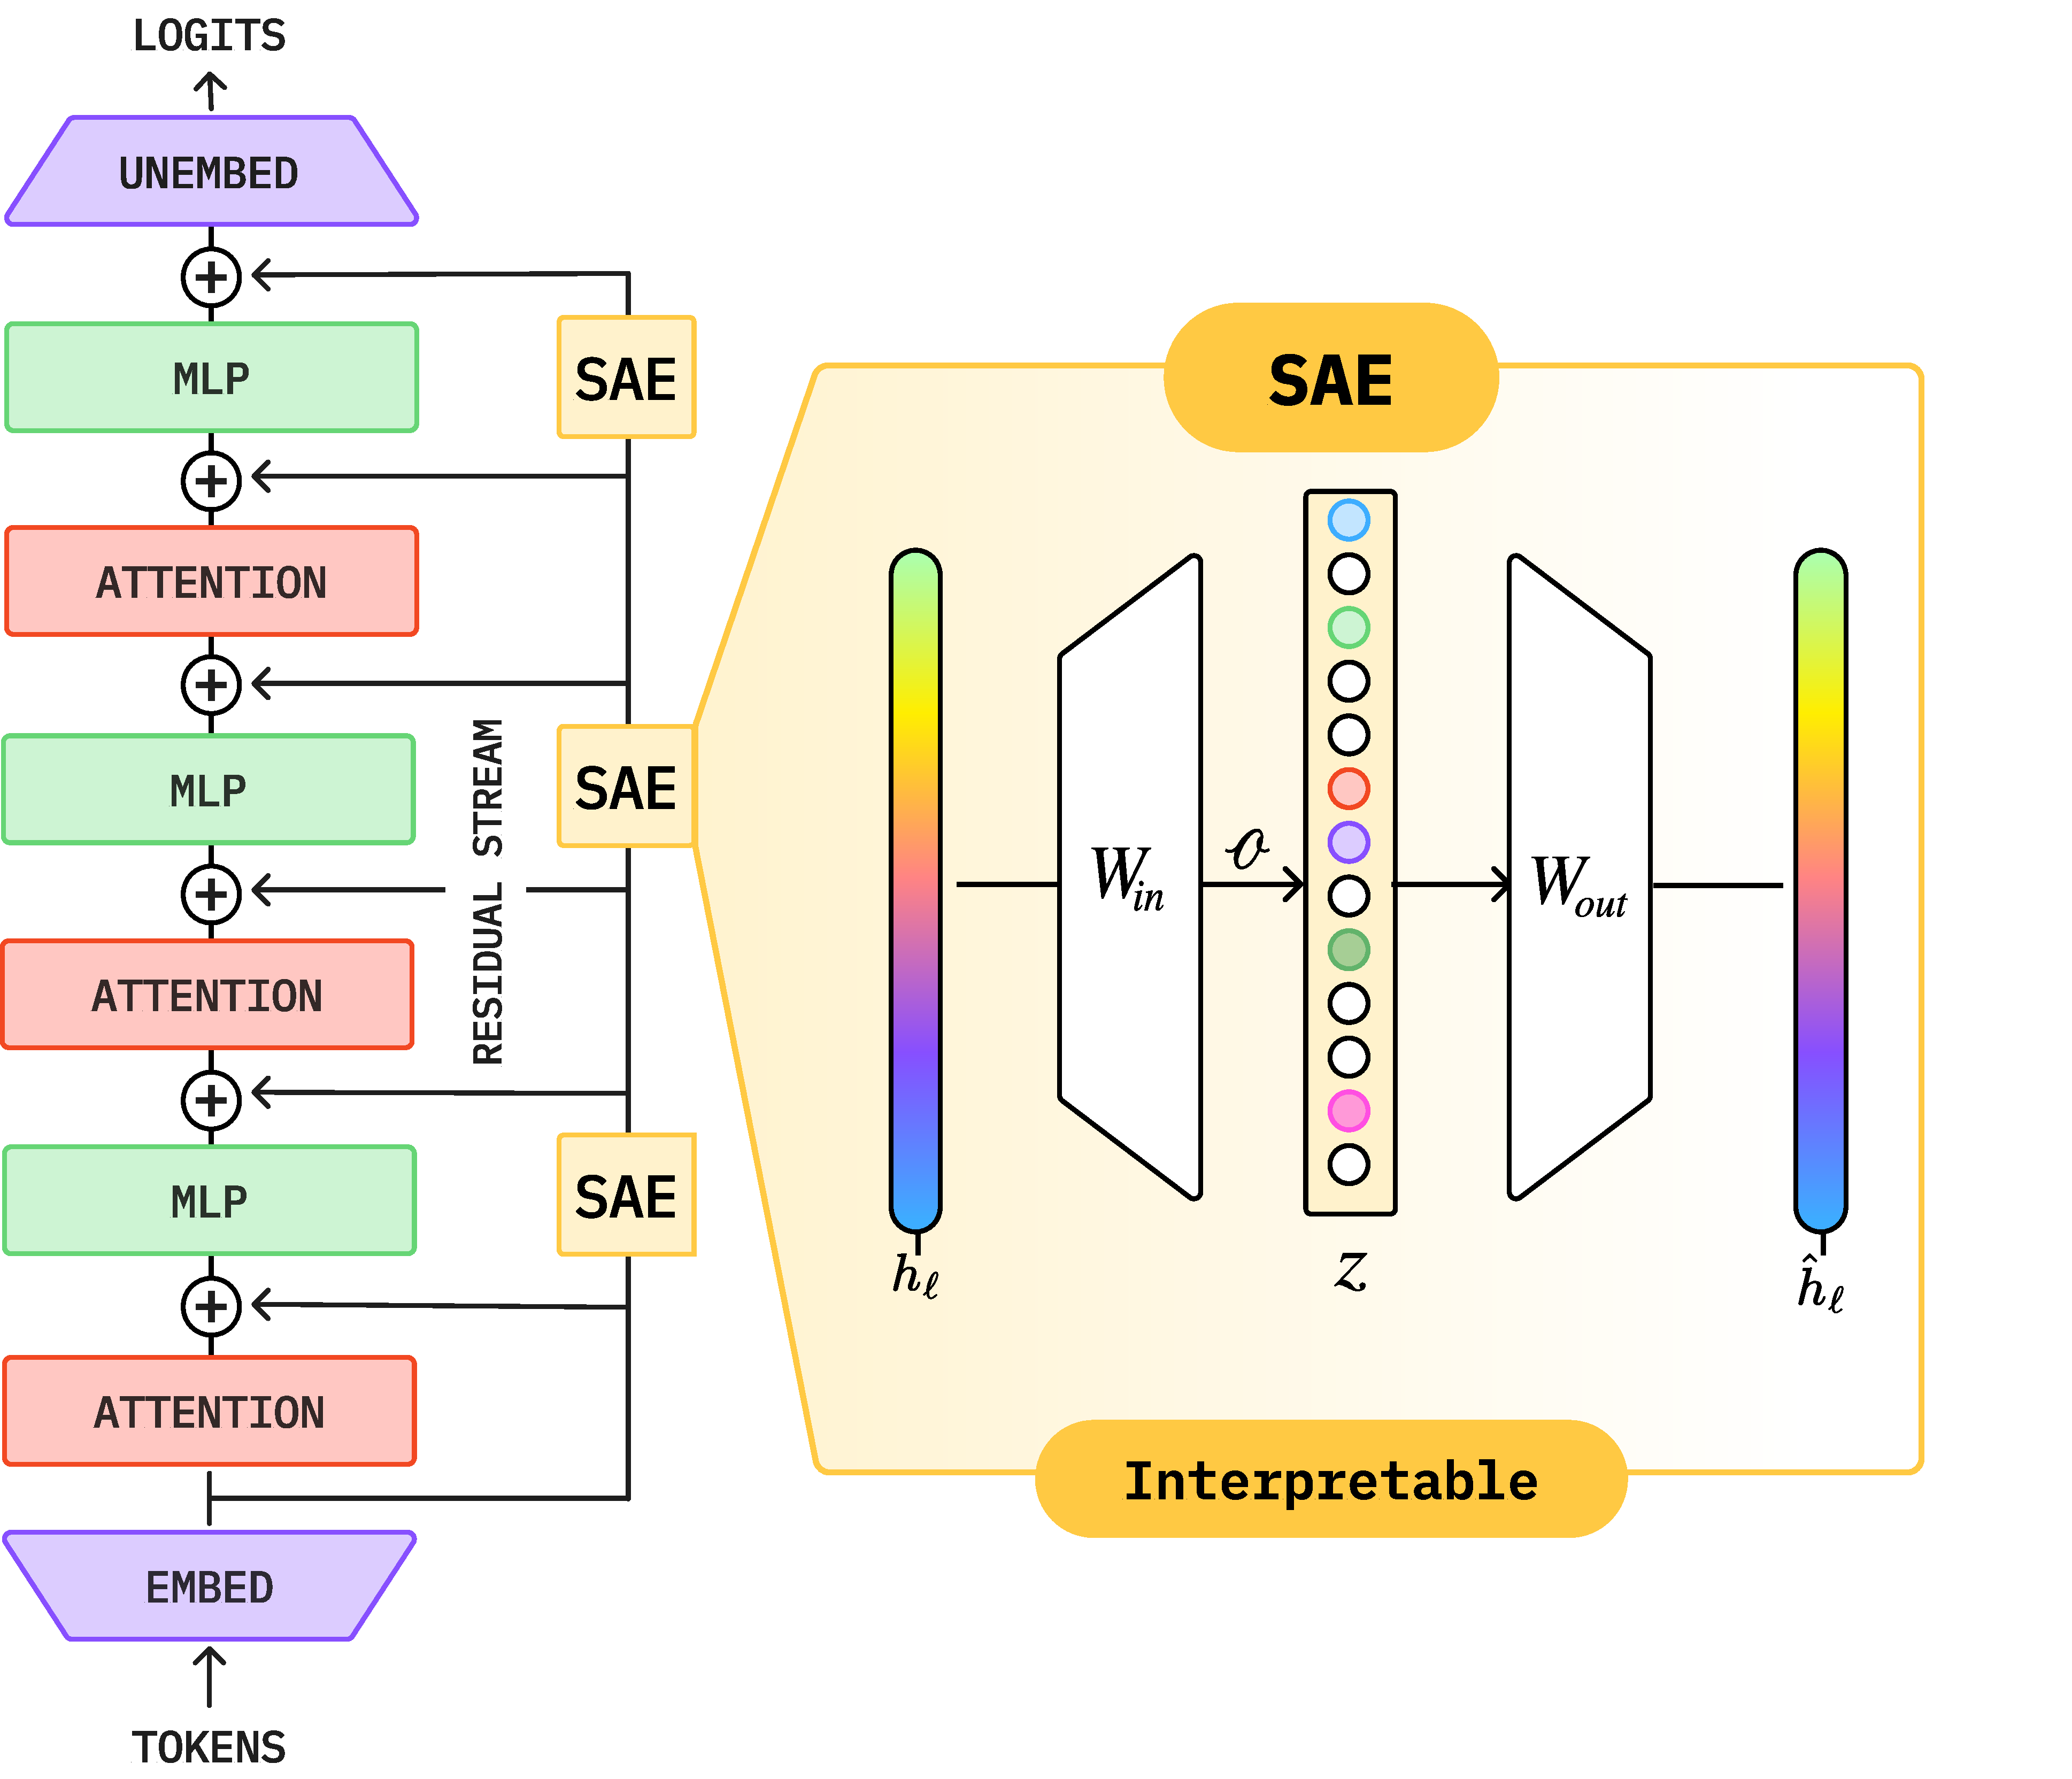
\includegraphics[width=0.8\linewidth]{figs/6_SAE.pdf}
    \caption{\textbf{Sparse Autoencoder (SAE).} SAEs are trained to reconstruct activations of a model component at a specific layer $\ell$, $h_\ell$, into an overcomplete, sparse latent space $z$, such that the reconstructed activation $\hat{h_\ell} \approx h_\ell$. By enforcing sparsity on $z$, the model decomposes dense, polysemantic representations into monosemantic, human-interpretable features.}
    \label{fig:sae}
\end{figure}

\begin{definitionbox}[Sparse Autoencoder (Figure~\ref{fig:sae})]
A sparse autoencoder learns a component-specific encoder--decoder pair
\[
E : \mathbb{R}^d \rightarrow \mathbb{R}^{d_{\text{sparse}}},
\qquad
D : \mathbb{R}^{d_{\text{sparse}}} \rightarrow \mathbb{R}^d,
\]
such that activations of a particular model component at a given layer, \(h_\ell \in \mathbb{R}^d\) (e.g., the output of the layer-\(\ell\) MLP block), are reconstructed as
\[
\hat{h}_\ell = D(E(h_\ell)),
\]
while encouraging the feature activations \(z=E(h_\ell)\) to be sparse. Usually, $d_{\text{sparse}} = ed$, where $e$ is an integer expansion factor.
\end{definitionbox}

\paragraph{Canonical Formulation.}
Given activations of a model component \( h_\ell \sim \mathcal{H} \), where $\mathcal{H}$ is the distribution of that component's activations over a large corpus, the canonical SAE objective is
\[
\mathcal{L}_{\text{SAE}}
=
\mathbb{E}_{h_\ell \sim \mathcal{H}}
\left[
\| h_\ell - D (z) \|_2^2
+ \lambda \| z \|_1
\right],
\quad
z = E(h_\ell),
\]
where $\lambda > 0$ controls sparsity~\citeest{cunningham2023sparse}. Canonical SAEs use $L_1$ regularisation instead of $L_0$ regularisation. This is because, for each feature, $L_0$'s derivative is almost everywhere zero and thus does not provide useful signals for promoting feature sparsity during gradient descent. Additionally, the decoder columns are typically constrained to unit norm. This is to prevent the case where the SAE learns to reduce its $L_1$ loss by generating smaller values of $z$---not exactly $0$ so that many features can be active, each having a small coefficient---and enlarging the norm of each column of the decoder to compensate. In this way, the SAE output remains the same, while $L_1$ loss can be substantially reduced, without any real gain in sparsity.

\paragraph{Why SAEs Work.}
SAEs are motivated by the hypothesis that a model's activations can be approximated as linear combinations of many latent feature directions, which can be regarded as an extension of the linear representation hypothesis discussed in Section~\ref{subsec:linearity}. Sparsity means that only a small number of features are active for any given token or input, but not that the hidden state itself is sparse. Early sparse dictionary learning studies~\citeest{olshausen1996emergence, lewicki2000learning, aharon2006k} give us fair confidence that, if the hypothesis holds, dictionary learning can recover the structure as an overcomplete dictionary. These findings motivate using SAEs as a modern adaptation to extract monosemantic directions from the activations of neural networks~(\citeestalp{cunningham2023sparse}; \citeemalp{bricken2023monosemanticity}).



\paragraph{From Monosemanticity to Concept Identification.}
For each input activation, the raw SAE outputs are just a small set of vectors. Practical interpretability requires identifying the semantic concepts these vectors correspond to in natural language (so that they become human-understandable features). Empirically, SAE features selectively activate on structured token patterns that recur across input sequences, suggesting sensitivity to specific abstract semantic, functional, or lexical concepts~\citeem{marks2024enhancingneuralnetworkinterpretability}. Automated analysis pipelines~\citeest{gur-arieh-etal-2025-enhancing, paulo2025automatically} aggregate highly activating inputs to infer the concept each feature captures (see Section~\ref{sec:automated-interp} for a detailed discussion).

\paragraph{Training Dynamics and Evaluation.}
SAE training is sensitive to initialisation, sparsity strength, and decoder normalisation. Without proper constraints and hyperparameters, the features may collapse, duplicate, or absorb one another. SAEs are typically evaluated for reconstruction loss (fidelity of activation reconstruction), feature absorption (how often a general feature fails to fire because a more specific feature has absorbed its direction), and downstream test loss recovery (whether replacing activations with reconstructions preserves model behaviour). Together, these metrics assess both the quality of the decomposition and its mechanistic relevance to the original model's computation.

\subsection{SAE Variants and Architectural Improvements}
\label{subsec:sae-variants}

There are several variants of the standard SAE. One key reason to use alternatives is that standard SAE training penalises activation magnitude, which can lead to low activation even when a feature is clearly present (the shrinkage effect). Different optimisation frameworks also have different tunable parameters. The choice depends on the analysis goal, target layer type, model size, and budget constraints. 


\begin{definitionbox}[Gated SAEs]
Gated SAEs introduce multiplicative gates to decouple feature selection from magnitude:
\[
z = \underbrace{\mathbbm{1} \left( (W_{\text{gate}} h_\ell + b_{\text{gate}}) > 0 \right)}_{\text{Gating Path}} \odot \underbrace{\sigma_{\text{ReLU}}(W_{\text{in}} h_\ell + b_{\text{in}})}_{\text{Magnitude Path}},
\]
where $h_\ell \in \mathbb{R}^d$ denotes activations at layer $\ell$, $W_{\text{in}} \in \mathbb{R}^{{d_{\text{sparse}}} \times d}$ and $b_{\text{in}} \in \mathbb{R}^{d_{\text{sparse}}}$ are encoder $E$ parameters, $W_{\text{gate}} \in \mathbb{R}^{{d_{\text{sparse}}} \times d}$ and $b_{\text{gate}} \in \mathbb{R}^{d_{\text{sparse}}}$ are the gate parameters, and $\odot$ denotes element-wise product. This mitigates shrinkage effects induced by the $L_1$ penalty~\citeest{rajamanoharan2024improvingdictionarylearninggated}.
\end{definitionbox}

\noindent
\begin{minipage}[c]{0.65\textwidth}
    \begin{definitionbox}[JumpReLU SAEs]
    JumpReLU SAEs~\citeem{rajamanoharan2024jumpingaheadimprovingreconstruction} learn per-feature activation thresholds. Given the encoder pre-activation $a = W_{\text{in}} h_\ell + b_{\text{in}}$, let $a_i$ denote its $i$-th entry. The activation value of the $i$-th feature after applying JumpReLU is
    \[
    z^i = \sigma_{\text{JumpReLU}}(a_i) = \begin{cases} 
    a_i & \text{if } a_i > \tau_i \\ 
    0 & \text{otherwise},
    \end{cases}
    \]
    where $\tau_i$ is a learned threshold parameter. Straight-through estimators~\citeem{bengio2013estimatingpropagatinggradientsstochastic} are used during training to enable gradient flow.
    \end{definitionbox}
\end{minipage}
\hfill
\begin{minipage}[c]{0.30\textwidth}
\vspace{0.5cm}
\hspace{-0.5cm}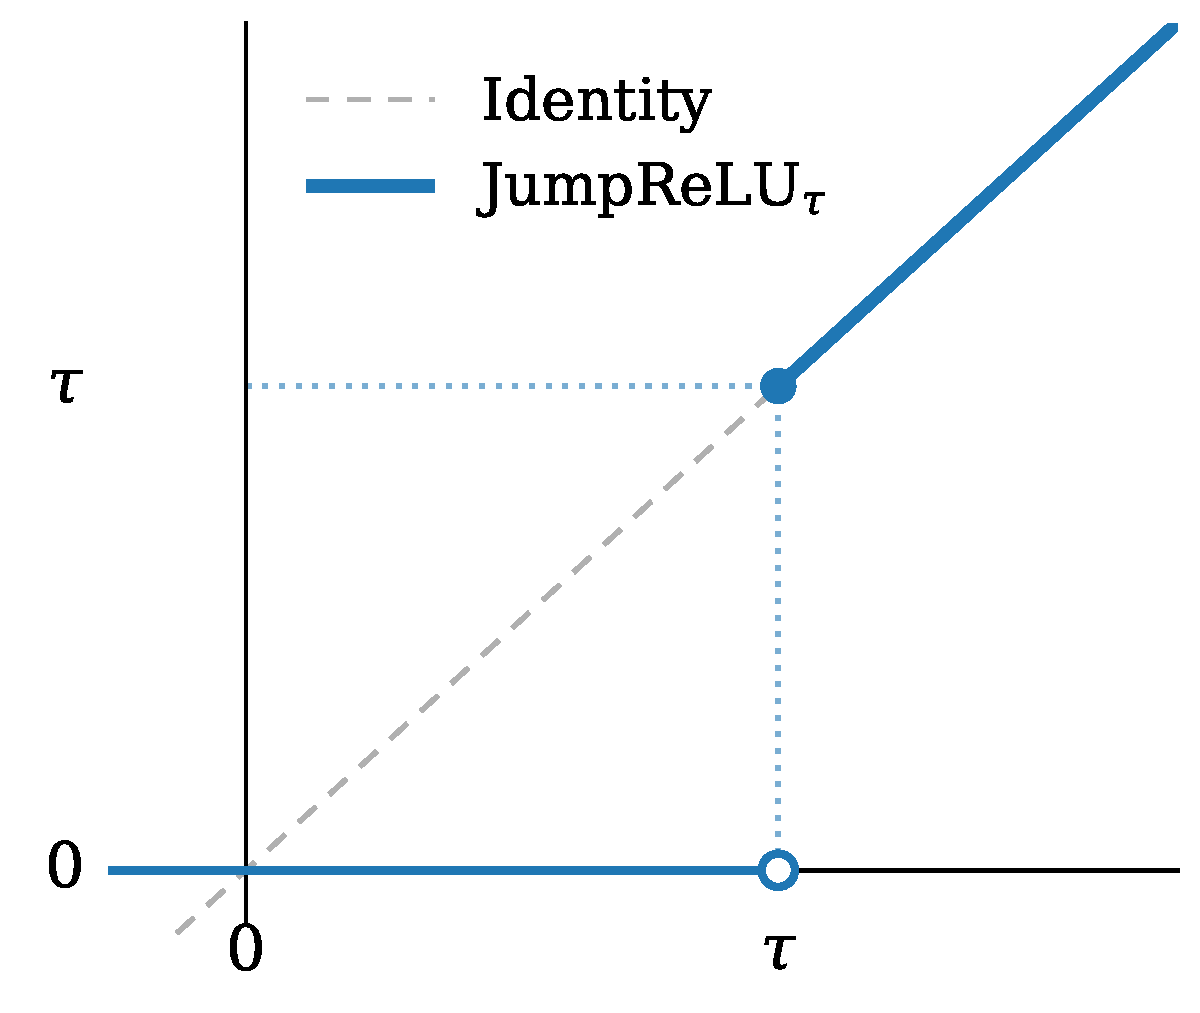
\includegraphics[width=1.\textwidth]{figs/JumpReLU.pdf}
\end{minipage}


\begin{definitionbox}[Top-$k$ SAEs]
Top-$k$ SAEs~\citeest{gao2024scalingevaluatingsparseautoencoders} impose an explicit hard sparsity constraint. Let $a = W_{\text{in}} h_\ell + b_{\text{in}} \in \mathbb{R}^{d_{\text{sparse}}}$ denote encoder pre-activations. Top-$k$ SAEs define the $i$-th feature's activation as
\[
z^i = \sigma_{\text{TopK}}(a_i) = \begin{cases}
a_i & \text{if } i \in \mathcal{I}_k(a) \\
0 & \text{otherwise},
\end{cases}
\]
where $\mathcal{I}_k(a)$ indexes the $k$ largest entries of $a$. This formulation explicitly enforces $\|z\|_0 \le k$---a more direct feature-sparsity constraint than $L_1$ regularisation. Notably, as it does not suppress activation magnitudes, it avoids the feature-shrinkage issue observed in $L_1$-based SAE training~\citeest{gao2024scalingevaluatingsparseautoencoders}.
\end{definitionbox}

\begin{definitionbox}[Batch Top-$k$ SAEs]

Batch Top-$k$ SAEs relax the fixed per-example sparsity constraint of standard Top-$k$ SAEs by enforcing the sparsity budget across an entire batch instead~\citeem{bussmann2024batchtopksparseautoencoders}. For a batch of encoder activations
\[
\big[\, a^{(1)}, \dots, a^{(B)} \,\big] \in \mathbb{R}^{d_{\text{sparse}} \times B},
\]
where $B$ is the batch size, Batch Top-$k$ retains the largest $Bk$ activation values in the batch. Specifically, let
\[
\mathcal{I}
\coloneqq
\arg\max_{\substack{
\mathcal{S}\subseteq
\{1,\ldots,B\}\times
\{1,\ldots,d_{\text{sparse}}\}\\
|\mathcal{S}|=Bk
}}
\sum_{(b,j)\in\mathcal{S}}
a_j^{(b)}.
\]
In each batch, the activation value of the $j$-th feature in the $b$-th sample is
\[
z^{j, (b)}
=
\sigma_{\text{Batch-TopK}}\!\left(a_j^{(b)}\right)
=
\begin{cases}
a_j^{(b)}, & (b,j)\in\mathcal{I},\\
0, & \text{otherwise}.
\end{cases}
\]

That is, each batch exactly retains $Bk$ features, while individual samples may have more or fewer active features than $k$. This loose constraint allows the model to allocate representational capacity adaptively across samples. During inference, Batch Top-$k$ SAEs instead use the JumpReLU function with an inferred global threshold to determine which features are active for each input, so that an input's activations do not depend on the rest of the batch.
\end{definitionbox}


\begin{insightbox}[Trade-offs Between Variants]
Different SAE variants may implement distinct sparsity constraints. No single variant is optimal across all scenarios.\\

\begin{center}
\small
\begin{tabular}{lccc}
\toprule
\textbf{Variant} & \textbf{Sparsity} & \textbf{Differentiable} & \textbf{Tuning Required} \\
\midrule
$L_1$-regularised & Soft & \cmark & $\lambda$ coefficient \\
Gated & Learned & \xmark$^\dagger$ & $\lambda$ coefficient \\
JumpReLU & Learned & \xmark$^*$ & $\lambda$ coefficient, STE bandwidth, threshold init. \\
Top-$k$ & Hard & \xmark & $k$ value \\
Batch Top-$k$ & Hard & \xmark & $k$ value \\
\bottomrule
\end{tabular}
\end{center}
\vspace{0.5em}
{\small $^*$Uses straight-through estimators (STEs) during training. $^\dagger$Trains the non-differentiable gate with auxiliary losses.}
\end{insightbox}
Readers are referred to \citetest{shu-etal-2025-survey} for a dedicated survey of SAEs, their variants, evaluations, and applications. Additionally, researchers have published SAE weights for several language models, including Gemma Scope~\citeem{lieberum2024gemmascopeopensparse} for Gemma 2~\citeem{gemmateam2024gemma2improvingopen} and Llama Scope~\citeem{he2024llamascopeextractingmillions} for Llama-3.1-8B~\citeem{llama3}. They can be accessed through open platforms such as Neuronpedia~\citeem{neuronpedia}.

\subsection{Empirical Comparisons of SAE Variants}
\label{subsec:sae-selection}

The SAE variants in Section~\ref{subsec:sae-variants} differ principally in how they enforce
sparsity, and those differences map onto distinct analysis settings. 

Hard-constraint formulations (e.g., Top-$k$) directly enforce sparsity and suit tight compute budgets. Learned-threshold (e.g., JumpReLU SAE) and gated formulations usually achieve better reconstruction results and suit generous tuning budgets. Cross-layer variants (discussed in Section~\ref{subsec:transcoders-crosscoders}) analyse computations across layers that a single dictionary cannot represent at all. This subsection discusses the setting in which each variant is used and the evidence it provides. We particularly discuss four factors that account for most of the variation:

\begin{enumerate}
    \item \textbf{Analysis goal:} exploratory discovery vs.\ targeted investigation vs.\ deployment/monitoring
    \item \textbf{Layer type:} residual stream vs.\ MLP output vs.\ attention output
    \item \textbf{Model scale:} small ($<$1B) vs.\ medium (1--10B) vs.\ large ($>$10B parameters)
    \item \textbf{Resource constraints:} compute budget, hyperparameter tuning capacity, tolerance for training instability
\end{enumerate}

\paragraph{Analysis Goal.}
\emph{Exploratory discovery}, where the question is what features exist rather than whether
a particular one does, is the setting SAEs were designed for and the one the comparisons
below address. For \emph{targeted investigation} of an already-identified behaviour, where the concepts of interest are determined, supervised methods such as DAS~\citeest{das} and linear probes are more direct instruments. For \emph{online deployment and monitoring}, SAEs with small dictionaries can be preferable for low inference cost.

\paragraph{Layer Type.}
Layer types differ in their activation properties, so the right variant depends on what each can represent, not just how well. On the \emph{residual stream}, single-layer SAEs
apply directly, and the choice reduces to the resource considerations below. On \emph{MLP
outputs}, transcoders are the appropriate tool: a single-layer SAE cannot span the
nonlinearity, so transcoders learn the input-to-output map
directly~\citeest{dunefsky2024transcodersinterpretablellmfeature}, and
\citetem{paulo2025transcodersbeatsparseautoencoders} reported favourable comparisons against
SAEs there. On \emph{attention outputs}, standard and Gated SAEs both have been used;
attention-specific variants remain underdeveloped, making this the least studied of the three
sites. For \emph{cross-layer analysis}, crosscoders~\citeem{lindsey2024sparsecrosscoders}
and cross-layer transcoders~\citeem{ameisen2025circuit} track feature evolution across
layers at substantially higher compute cost, and a crosscoder trained jointly on two models
is the reported approach for comparing representations between them. Table~\ref{tab:sae-layer-recommendations} summarises the variants used at each layer type, the empirical rationale for their use, and the main caveats reported in prior work.

\begin{table}[tb]
\centering
\caption{Heuristic recommendations for selecting SAE variants across different layer types. Recommendations are based on current empirical evidence and practical experience, and may evolve as SAE methodologies and evaluation standards continue to develop.}
\label{tab:sae-layer-recommendations}
\renewcommand{\arraystretch}{1.3}
\begin{tabular}{>{\raggedright\arraybackslash}p{2.8cm} >{\raggedright\arraybackslash}p{3.2cm} >{\raggedright\arraybackslash}p{4cm} >{\raggedright\arraybackslash}p{4cm}}
\toprule
\rowcolor{tableheader!80} \textcolor{white}{\textbf{Layer Type}} & \textcolor{white}{\textbf{Variants Used}} & \textcolor{white}{\textbf{Reported Basis}} & \textcolor{white}{\textbf{Reported Caveats}} \\
\midrule
\rowcolor{tablerow1} Residual stream (early layers) & Gated SAE, Top-$k$ & Activations are closer to input embeddings; moderate sparsity & Smaller expansion factors (2--4$\times$) reported \\
\rowcolor{tablerow2} Residual stream (middle layers) & Gated SAE, JumpReLU & Richest feature structure; highest interpretability potential & Standard expansion factor (4--8$\times$); most studied regime \\
\rowcolor{tablerow1} Residual stream (late layers) & Top-$k$, Gated SAE & Activations increasingly task-specific; may be less sparse & Larger expansion factors (8--16$\times$) reported \\
\rowcolor{tablerow2} MLP outputs & Transcoder (Section~\ref{subsec:transcoders-crosscoders}) & MLP applies a nonlinearity a single-layer SAE cannot span & Not a sparse decomposition on a static object; bridges input to output $\ell$ \\
\rowcolor{tablerow1} Attention outputs & Gated SAE, standard SAE & Attention outputs often lower-rank & Least studied of the three sites; may benefit from smaller dictionaries \\
\rowcolor{tablerow2} Cross-layer & Crosscoder, CLT (Section~\ref{subsec:transcoders-crosscoders}) & Tracks feature evolution; resolves cross-layer superposition & High compute cost; requires multi-layer training \\
\bottomrule
\end{tabular}
\end{table}


\paragraph{Resource Constraints.}
Under limited compute, or where fast iteration matters more than reconstruction quality,
Top-$k$ SAEs~\citeest{gao2024scalingevaluatingsparseautoencoders} are the practical choice:
fixing $\|z\|_0 \le k$ removes the sparsity coefficient $\lambda$ from the search space
entirely rather than requiring it to be tuned, with reported values commonly in the range
$k = 32$~\citeest{gao2024scalingevaluatingsparseautoencoders} to $150$~\citeest{karvonen2025saebench}. With moderate tuning capacity, Gated
SAEs~\citeest{rajamanoharan2024improvingdictionarylearninggated} achieved a better
reconstruction--sparsity trade-off while retaining $\lambda$. They also avoid the shrinkage effect by separating feature detection from magnitude estimation. However, because the standard $L_1$ SAE is now used mainly as a baseline, comparisons against it partly reflect shrinkage rather than dictionary quality alone. When extensive tuning is plausible, JumpReLU
SAEs~\citeem{rajamanoharan2024jumpingaheadimprovingreconstruction} achieved the strongest reconstruction performance at matched sparsity by learning per-feature thresholds. However,
gains on these sparsity--fidelity proxy metrics do not reliably translate
into better downstream performance~\citeest{karvonen2025saebench}. In practice, selecting the best model and hyperparameters to achieve optimal performance can take a lot of time.

\paragraph{Model Scale.}
The differences between variants depend strongly on the metric in models with roughly 1 or 2B parameters, such as Gemma-2-2B~\citeest{karvonen2025saebench}, which is the regime mainly used to validate methodology before scaling. For models between 1B and 10B parameters, JumpReLU SAEs and Top-$k$ SAEs are the most commonly reported variants; Gemma Scope~\citeem{lieberum2024gemmascopeopensparse} uses the former and Llama Scope~\citeem{he2024llamascopeextractingmillions} the latter. For models larger than 10B parameters, Gemma Scope~\citeem{lieberum2024gemmascopeopensparse} (for Gemma 2 models) and Gemma Scope 2~\citeem{mcdougall2025gemmascope2} (for Gemma 3 models) are the main open resources, both of which used JumpReLU SAEs. Additionally, \citetest{gao2024scalingevaluatingsparseautoencoders} explored scaling Top-$k$ SAEs to GPT-4~\citeem{openai2024gpt4technicalreport}, although GPT-4 itself is not publicly available.

Table~\ref{tab:sae_recommendations} summarises each variant’s main findings reported in previous work, along with their experimental settings. Note that these studies may use different baselines, model families, sparsity constraints, and evaluation criteria. The community has been establishing benchmarks to evaluate variants of SAEs, such as SAEBench~\citeest{karvonen2025saebench}, but the results vary by metric. As a result, we should treat the findings as references rather than established rules. The \emph{Setting} column in Table~\ref{tab:sae_recommendations} records the conditions under which each result is established. Table~\ref{tab:sae_limitations} further highlights several factors that limit the generality of the findings.

\begin{table}[tb]
\centering
\caption{Reported evidence for each SAE variant, with the setting in which it was obtained.}
\label{tab:sae_recommendations}
\renewcommand{\arraystretch}{1.3}
\begin{tabular}{>{\raggedright\arraybackslash}p{2.4cm} >{\raggedright\arraybackslash}p{6.2cm} >{\raggedright\arraybackslash}p{4.6cm}}
\toprule
\rowcolor{tableheader!80} \textcolor{white}{\textbf{Variant}} & \textcolor{white}{\textbf{Reported Finding}} & \textcolor{white}{\textbf{Setting}} \\
\midrule
\rowcolor{tablerow1} Standard & Sparse dictionary learning by $L_1$ regularisation recovers features more monosemantic than individual neurons; subject to shrinkage bias & Establishing work, small models~(\citeestalp{cunningham2023sparse}; \citeemalp{bricken2023monosemanticity}) \\
\rowcolor{tablerow2} Gated & Separating detection from magnitude estimation addresses $L_1$ shrinkage at minimal added complexity & Reconstruction--sparsity improvement at matched sparsity, Gemma-family~\citeest{rajamanoharan2024improvingdictionarylearninggated} \\
\rowcolor{tablerow1} JumpReLU & Learned per-feature thresholds trained with straight-through estimators give the strongest reported reconstruction & Matched-sparsity comparison, Gemma-family~\citeem{rajamanoharan2024jumpingaheadimprovingreconstruction}; needs most tuning~\citeem{bussmann2024batchtopksparseautoencoders} \\
\rowcolor{tablerow2} Top-$k$ & A hard $\|z\|_0 \le k$ constraint removes the sparsity coefficient from the search space & Scaling behaviour characterised on large models; $k = 32$--$150$ commonly reported~\citeest{gao2024scalingevaluatingsparseautoencoders, karvonen2025saebench} \\
\rowcolor{tablerow1} Batch Top-$k$ & A batch-level sparsity budget lets the number of active features vary per input, improving reconstruction at matched average sparsity & Introduced as a relaxation of per-example Top-$k$, achieving better reconstruction~\citeem{bussmann2024batchtopksparseautoencoders} \\
\rowcolor{tablerow2} Transcoder & Learning the MLP input--output map avoids spanning the nonlinearity with a single dictionary & Reported to perform at least on par with SAEs~(\citeestalp{dunefsky2024transcodersinterpretablellmfeature}; \citeemalp{paulo2025transcodersbeatsparseautoencoders}) \\
\rowcolor{tablerow1} Crosscoder & Joint reconstruction across layers tracks feature evolution and resolves cross-layer superposition & Cross-layer analysis and model diffing; trained jointly across models for cross-model comparison~\citeem{lindsey2024sparsecrosscoders} \\
\rowcolor{tablerow2} CLT & Partial reconstruction of multiple downstream layers from one dictionary & Deployed within CLT-based circuit discovery at scale~\citeem{ameisen2025circuit} \\
\bottomrule
\end{tabular}
\end{table}

\begin{table}[tb]
\centering
\caption{Conditions for the reported evidence on SAE variant behaviour.}
\label{tab:sae_limitations}
\renewcommand{\arraystretch}{1.3}
\begin{tabular}{>{\raggedright\arraybackslash}p{0.32\linewidth} >{\raggedright\arraybackslash}p{0.58\linewidth}}
\toprule
\rowcolor{tableheader!80} \textcolor{white}{\textbf{Condition}} & \textcolor{white}{\textbf{Description}} \\
\midrule
\rowcolor{tablerow1} Architecture dependence & Most evidence derives from Llama- and Gemma-family models. Generality of the findings across model families remains unestablished. \\
\rowcolor{tablerow2} Task dependence & The properties that matter may differ across analysis goals, such as safety auditing, behaviour understanding, and knowledge localisation, but existing evaluations often do not distinguish between them.\\
\rowcolor{tablerow1} Rapid iteration & New architectures and training procedures are proposed faster than existing ones are sufficiently studied and replicated. \\
\rowcolor{tablerow2} Immature theoretical analysis & Current findings are mostly empirical and may be superseded. Understanding of why particular variants succeed or fail is incomplete. \\

\rowcolor{tablerow1} Feature reproducibility & SAEs trained on the same data with different random seeds can recover substantially different features. When between-variant performance differences are smaller than within-variant seed-to-seed variability, we may not confidently attribute them to architectural factors. However, few reported comparisons have rigorously accounted for this concern. \\

\bottomrule
\end{tabular}
\end{table}



































\subsection{Challenges and Failure Modes of SAEs}
\label{subsec:challenge}

SAEs have become a standard tool for feature extraction, but they exhibit systematic failure modes that undermine their interpretability claims. It is therefore essential to understand these issues when using SAEs as mechanistic tools. This section provides a systematic discussion of them.

\subsubsection{Dead Features}
A \emph{dead feature} is an element in the learned dictionary that never activates or activates extremely rarely across training. Dead features waste the dictionary’s capacity, and they are common. In fact, they can constitute up to 10--50\% of the dictionary in a poorly tuned SAE~\citeem{bricken2023monosemanticity}. 

Several factors can cause dead features to emerge. First, inappropriate SAE weight initialisation can place features in low-density regions of the activation space with weak gradient signals. Second, an overly strong sparsity penalty $\lambda$ may suppress feature activations early in training, preventing features from contributing usefully to reconstruction. Finally, once a subset of features captures common, dominant patterns, the remaining features struggle to find useful roles for improving reconstruction and thus do not activate.

Dead features can be detected by tracking each feature’s rate of being activated during training. For example, features with an activation rate below 0.01\% may be considered dead (the threshold should adapt across scenarios). Several mitigation strategies have been proposed, such as \emph{neuron resampling}, which periodically reinitialises dead features using examples with high reconstruction error~\citeem{bricken2023monosemanticity}. The sparsity penalty can also be reduced early in training and increased gradually (i.e., a warm-up schedule). More recent Batch Top-$k$ SAEs allocate sparsity adaptively across samples, which allows more active features on complex inputs and fewer on easy ones~\citeem{bussmann2024batchtopksparseautoencoders}.

\subsubsection{Feature Duplication}
Feature duplication occurs when multiple features in the dictionary encode the same or similar concepts~\citeem{templeton2024scaling}, leading to potentially redundant features. Duplication can arise for several reasons: insufficient sparsity pressure, imbalanced training data, or an optimisation process that favours local minima with duplicated features. Duplication can be detected by computing pairwise cosine similarity between feature directions (i.e., decoder columns), where high similarity indicates potential redundancy. As duplicated features tend to activate together~\citeem{korznikov2025ortsaeorthogonalsparseautoencoders}, co-activation statistics may provide complementary evidence. 

\subsubsection{Feature Absorption and Splitting}

Another class of failure modes concerns feature granularity. \emph{Feature absorption} arises when semantically hierarchical features interact under the sparsity objective: a seemingly general (\emph{parent}) feature fails to activate on some inputs where it should because a more specific (\emph{child}) feature activates instead and has absorbed part of the parent's direction into its own decoder direction~\citeest{chanin2025absorption}. For example, a ``starts with S'' feature may fail to activate on the token ``short'', while a token-specific ``short'' feature with a partially overlapping direction activates instead. Absorption-induced false negatives make such a feature an unreliable detector of its concept. It can be detected by comparing the feature with a linear probe for the same concept: inputs on which the probe responds strongly, but the feature does not, while another active feature's direction aligns with the probe, indicate absorption~\citeest{chanin2025absorption}.

By contrast, \emph{feature splitting} occurs when a feature learned by a smaller SAE splits into multiple distinct features as the SAE scales up (e.g., by increasing the expansion factor \(e\)). This often produces more fine-grained features, which may be either beneficial or less useful. In a favourable case, an initially polysemantic or opaque feature, such as one activating on ``bank'' in both financial and geographical contexts, may split into more coherent features of ``investment bank'' and ``river bank''. In a less useful case, the resulting features may become low-level, lexical detectors that activate on the token ``bank'' in any context.

\subsubsection{Feature Instability Across Seeds}

SAE features are also sensitive to random initialisation, optimiser stochasticity, and data ordering. For a fixed SAE architecture and training dataset, different random seeds can produce substantially different dictionaries~\citeest{paulo2025sparse}. In practice, frequent and semantically clear features tend to be stable, while rare or context-specific features vary substantially. Often, fewer than 50\% of features remain the same across seeds, although broader semantic clusters may remain more consistent. This instability limits the reliability of mechanistic claims based on individual SAE features. Although aggregating results across seeds can improve robustness, it increases computational cost. As a result, when evaluating SAEs, we should report feature stability across seeds alongside reconstruction loss.

\subsubsection{Identifiability and Theoretical Concerns}
\label{subsubsec: sae limitation}
Another concern for SAE-based interpretability claims is whether the learned features are identifiable, that is, whether the dictionary learning reliably recovers the ``true'' underlying features---if such features exist---or merely finds one of many mediocre decompositions~\citeem{klindt2025superpositionsparsecodesinterpretable}.

\begin{definitionbox}[Identifiability]
Suppose activations are generated by some sparse latent process

\[
h = D^{*} z^{*} + \epsilon ,
\]

where \(D^{*}\) is the ground-truth feature dictionary and
\(z^{*}\) are the feature coefficients. An SAE is identifiable if its training recovers \(D^{*}\) and \(z^{*}\)
up to unavoidable symmetries such as feature permutation and rescaling.
\end{definitionbox}

In classical dictionary learning, identifiability holds under low-coherence conditions, i.e., dictionary elements are sufficiently orthogonal to one another. However, when coherence is high, ambiguity arises: multiple distinct sparse combinations of features from the same dictionary can generate the same output~\citeest{schnass2008dictionary}. In large language model activations, high coherence is likely unavoidable because of the model's complicated internal structure and correlations within its feature space~\citeest{li2025geometry}. So far, identifiability remains a stubborn issue in SAEs, even though it offers a theoretical explanation for several empirical observations.

Recent progress in fine-tuning language models around a fixed sparse autoencoder offers a potential path forward. In this setting, model activations are explicitly constrained to be sparse combinations of decoder features while largely preserving task performance~\citeest{chen2025low}. In particular, recent work aimed at limiting superposition fine-tunes the language model jointly with the SAE while enforcing orthogonality constraints on the decoder matrix~\citeem{miller2026identifyingintervenableinterpretablefeatures}. By explicitly imposing low-coherence conditions, this approach improves identifiability: activations have a unique feature representation, and these features can be reliably recovered.

\paragraph{Relation to Causal Relevance.}
The concern of identifiability connects to causal relevance: even if an SAE feature is monosemantic and helps reconstruct activations well, it may not correspond to a causally meaningful unit of analysis. Below, we summarise some criteria for validating an SAE feature.

\textbf{Diagnostic criteria:}
\begin{itemize}
    \item \textit{Necessity}: Does ablating the feature remove the corresponding concept in model responses? Low necessity suggests that the concept can be expressed through redundant features.
    \item \textit{Sufficiency}: Does activating only this feature produce the behaviour corresponding to its concept? Low sufficiency suggests the feature alone is not enough to represent the concept.
    \item \textit{Specificity}: Does the feature's causal effect match its corresponding concept? Low specificity means the feature contains other concepts.
\end{itemize}

These criteria are useful in practice when claiming that SAE features represent meaningful units of analysis.


\subsubsection{Practical Recommendations}
The challenges discussed above suggest several methodological considerations for SAE-based interpretability studies:

\begin{enumerate}
    \item \textbf{Report failure-mode metrics:} Alongside reconstruction loss, researchers should also report dead-feature percentage, duplication rate, and stability across seeds.
    
    \item \textbf{Validate causal relevance:} Researchers should validate features’ necessity, sufficiency, and specificity through interventions (e.g., feature ablation or steering) and evaluation on downstream effects. 
    
    \item \textbf{Compare methods:} For safety-critical applications, researchers should compare SAE features against various baselines to assess whether SAEs recover the relevant structure.
    
    \item \textbf{Try multiple SAE variants:} Different variants (e.g., Gated, Top-$k$, JumpReLU) impose different inductive biases. Researchers can explore findings consistent across variants, as these provide stronger evidence.
    
    \item \textbf{Acknowledge identifiability limits:} Researchers should frame SAE features as one valid approximate decomposition rather than the true features. Multiple decompositions may be equally valid for reconstruction but yield different feature sets.
    
    \item \textbf{Consider alternatives for targeted analysis:} When specific concepts are the focus, supervised methods (e.g., DAS, probes, discussed in Section~\ref{subsubsec: supervised_extraction}) may be more reliable because SAEs discover features in an unsupervised and exploratory manner.
\end{enumerate}


\subsection{Multi-Layer Feature Extraction and Analysis}
\label{subsec:transcoders-crosscoders}

Standard SAEs analyse individual layers in isolation. However, features can evolve as information propagates through the network. Transcoders (Figure~\ref{fig:transcoders}), cross-layer transcoders (Figure~\ref{fig:clt}), and crosscoders (Figure~\ref{fig:crosscoders}) enable multi-layer feature extraction and analysis, revealing how representations and features associated with particular model components---most commonly MLP blocks---transform across depth.

\subsubsection{Transcoders: Bridging the Nonlinearities}
\label{subsubsec:transcoder}

\begin{definitionbox}[Transcoder (Figure~\ref{fig:transcoders})]
A \emph{transcoder} learns a sparse mapping between the input to and output of a model component, such as an MLP block, in layer $\ell$:
\[
h_{\ell}^{\text{out}} \approx W_{\text{out}} z + b_{\text{out}}, \quad z = \sigma(W_{\text{in}} h_\ell^{\text{in}} + b_{\text{in}})
\]
where $z \in \mathbb{R}^{d_{\text{sparse}}}$ are sparse feature activations bridging the nonlinearity between input and output of the MLP, and $W_{\text{out}} \in \mathbb{R}^{d \times {d_{\text{sparse}}}}$ and $b_{\text{out}} \in \mathbb{R}^{d}$ are decoder $D$ parameters. The transcoder reconstructs post-nonlinearity activations using features extracted from pre-nonlinearity activations~\citeest{dunefsky2024transcodersinterpretablellmfeature}.
\end{definitionbox}

\paragraph{Architecture and Motivation.}
Standard SAEs do not explain the nonlinear transformations (i.e., weight matrices of MLP blocks and attention heads) themselves that produce the activations. A transcoder achieves this by applying dictionary learning to the mapping, learning features that explain the transformation. Its training minimises
\[
\mathcal{L} = \|h_{\ell}^{\text{out}} - (W_{\text{out}} z + b_{\text{out}})\|_2^2 + \lambda \|z\|_1,
\]
where $z = \sigma(W_{\text{in}} h^{\text{in}}_\ell + b_{\text{in}})$ as defined above. 
\paragraph{When Are Transcoders Necessary?}
SAEs extract features from static activations and thus often suffice for residual-stream analysis. Transcoders track how features emerge from input to output and are essential for analysing MLP layers~\citeest{dunefsky2024transcodersinterpretablellmfeature}.

\begin{figure}[tbp]
  \centering
  \begin{subfigure}{0.48\linewidth}
    \centering
    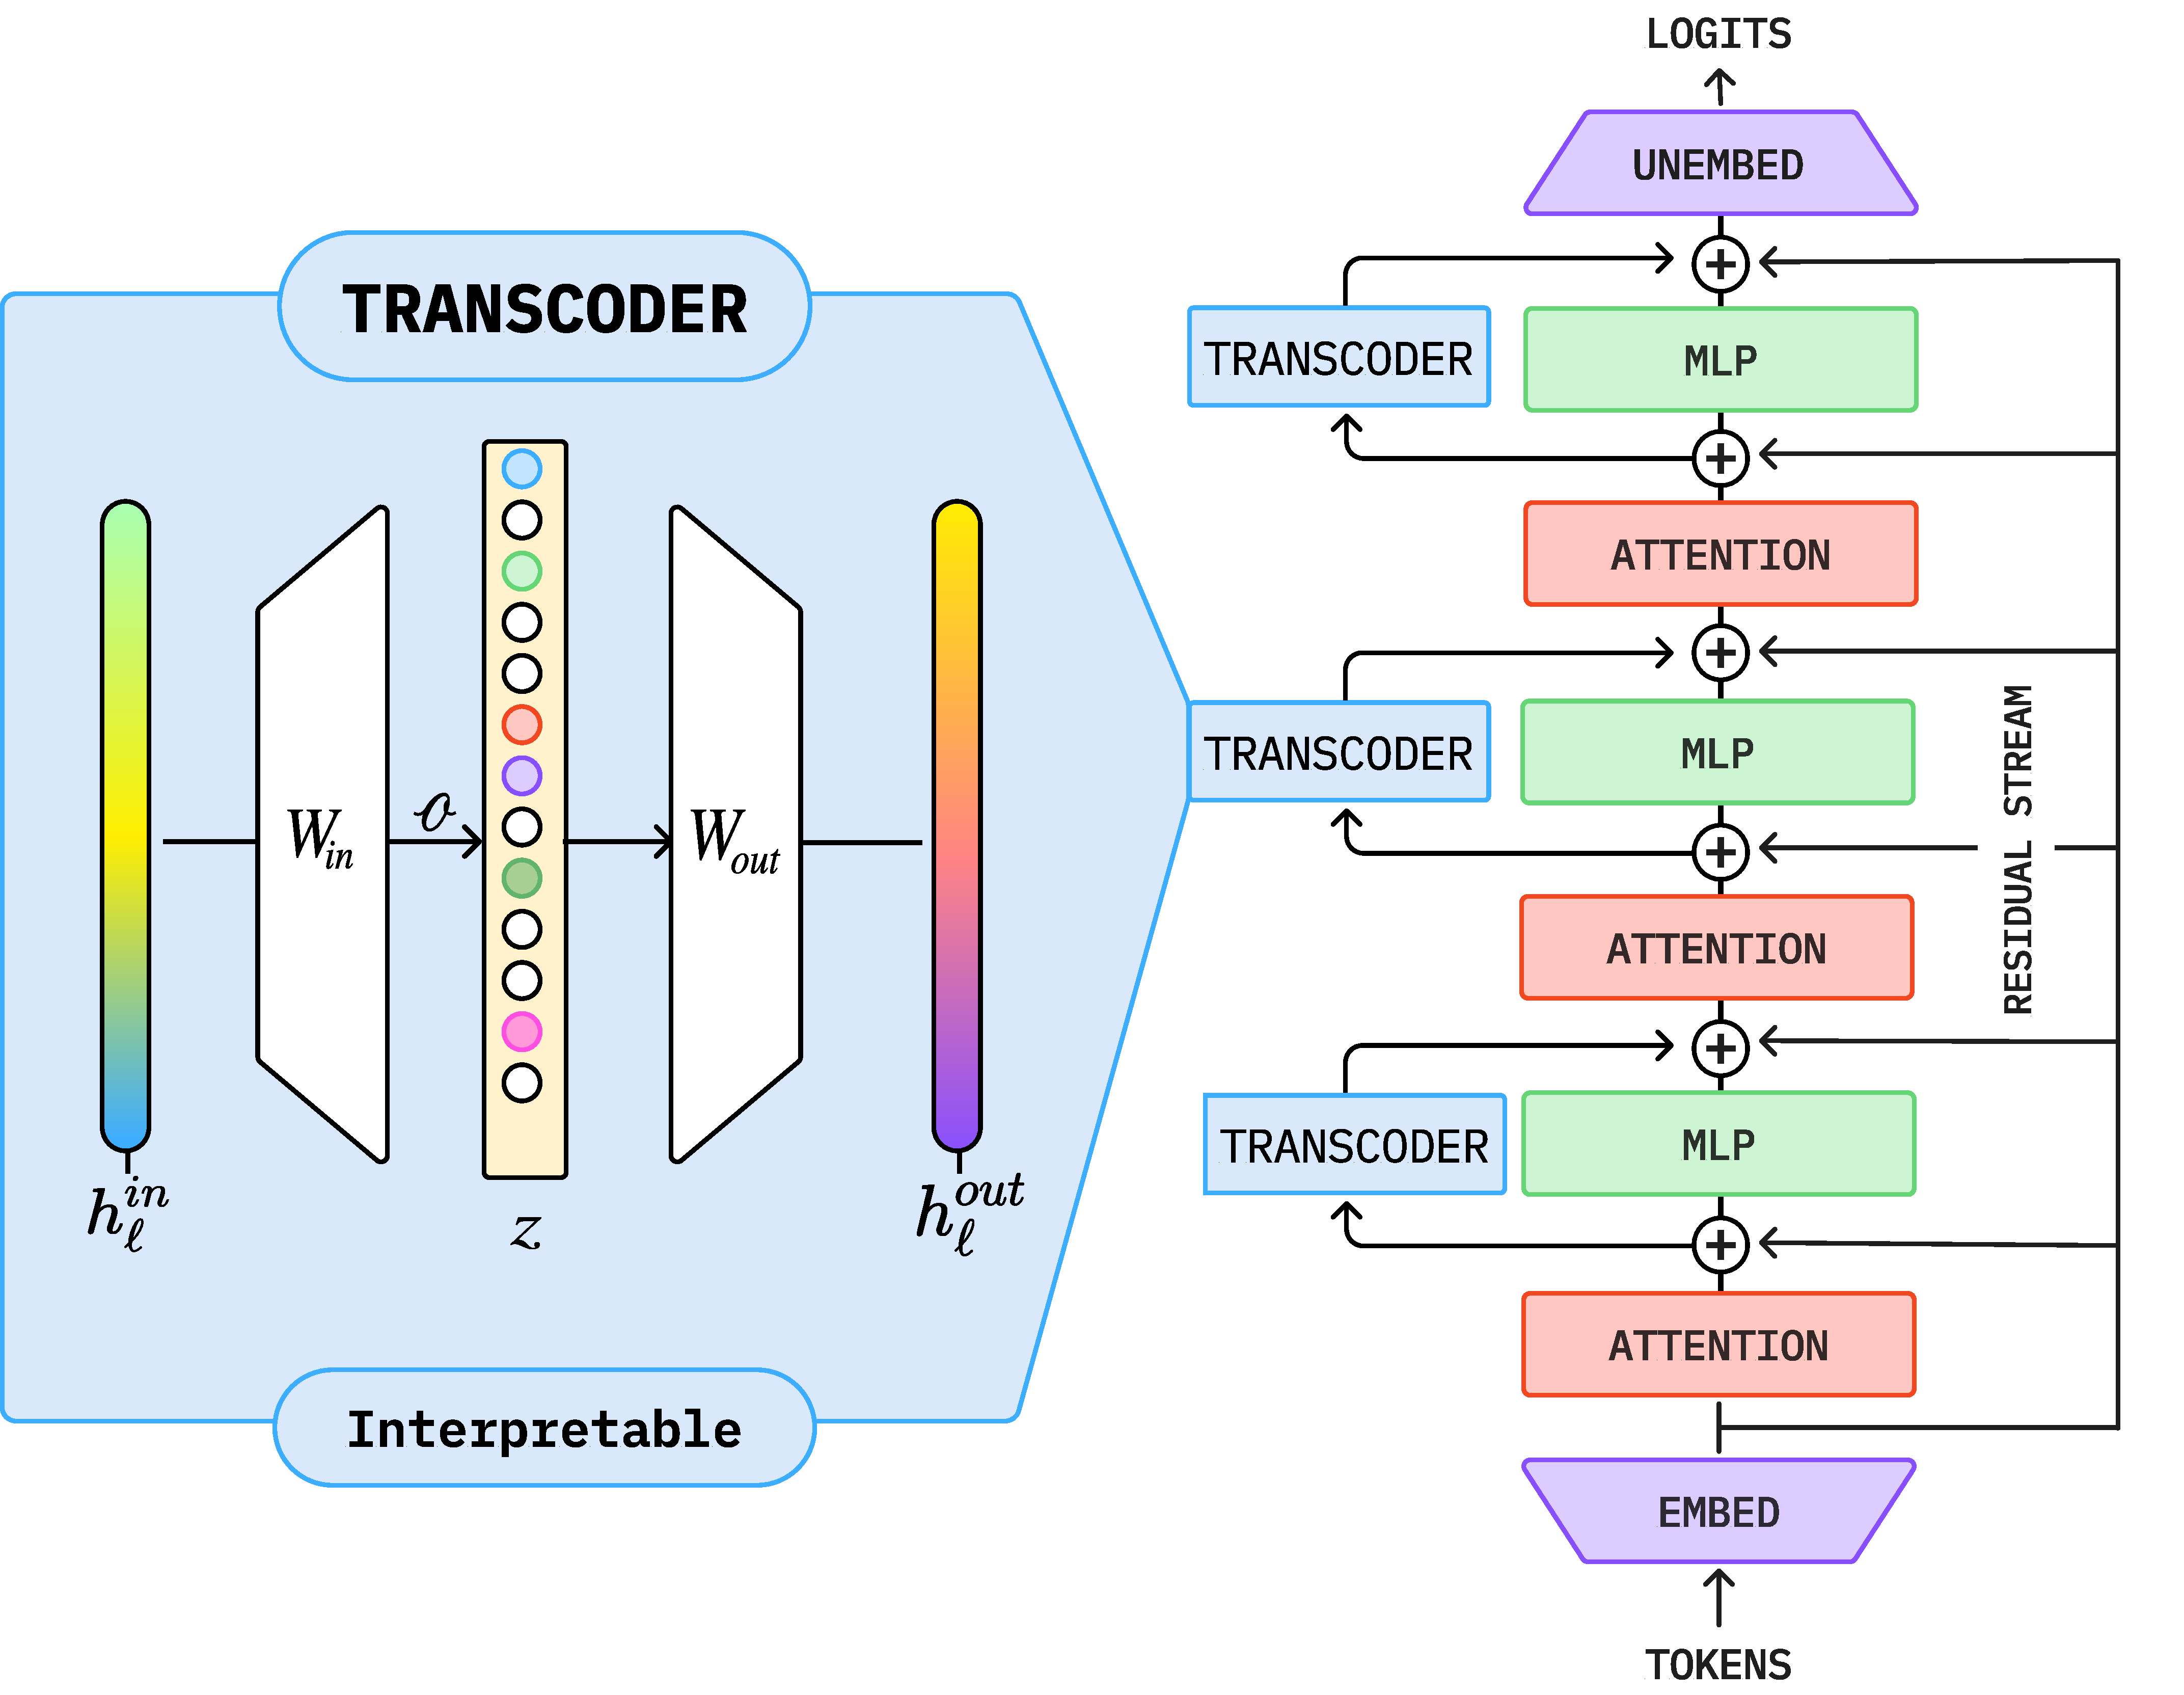
\includegraphics[width=\linewidth]{figs/6_Transcoders.pdf}
    \caption{Transcoder.}
    \label{fig:transcoders}
  \end{subfigure}\hfill
  \begin{subfigure}{0.48\linewidth}
    \centering
    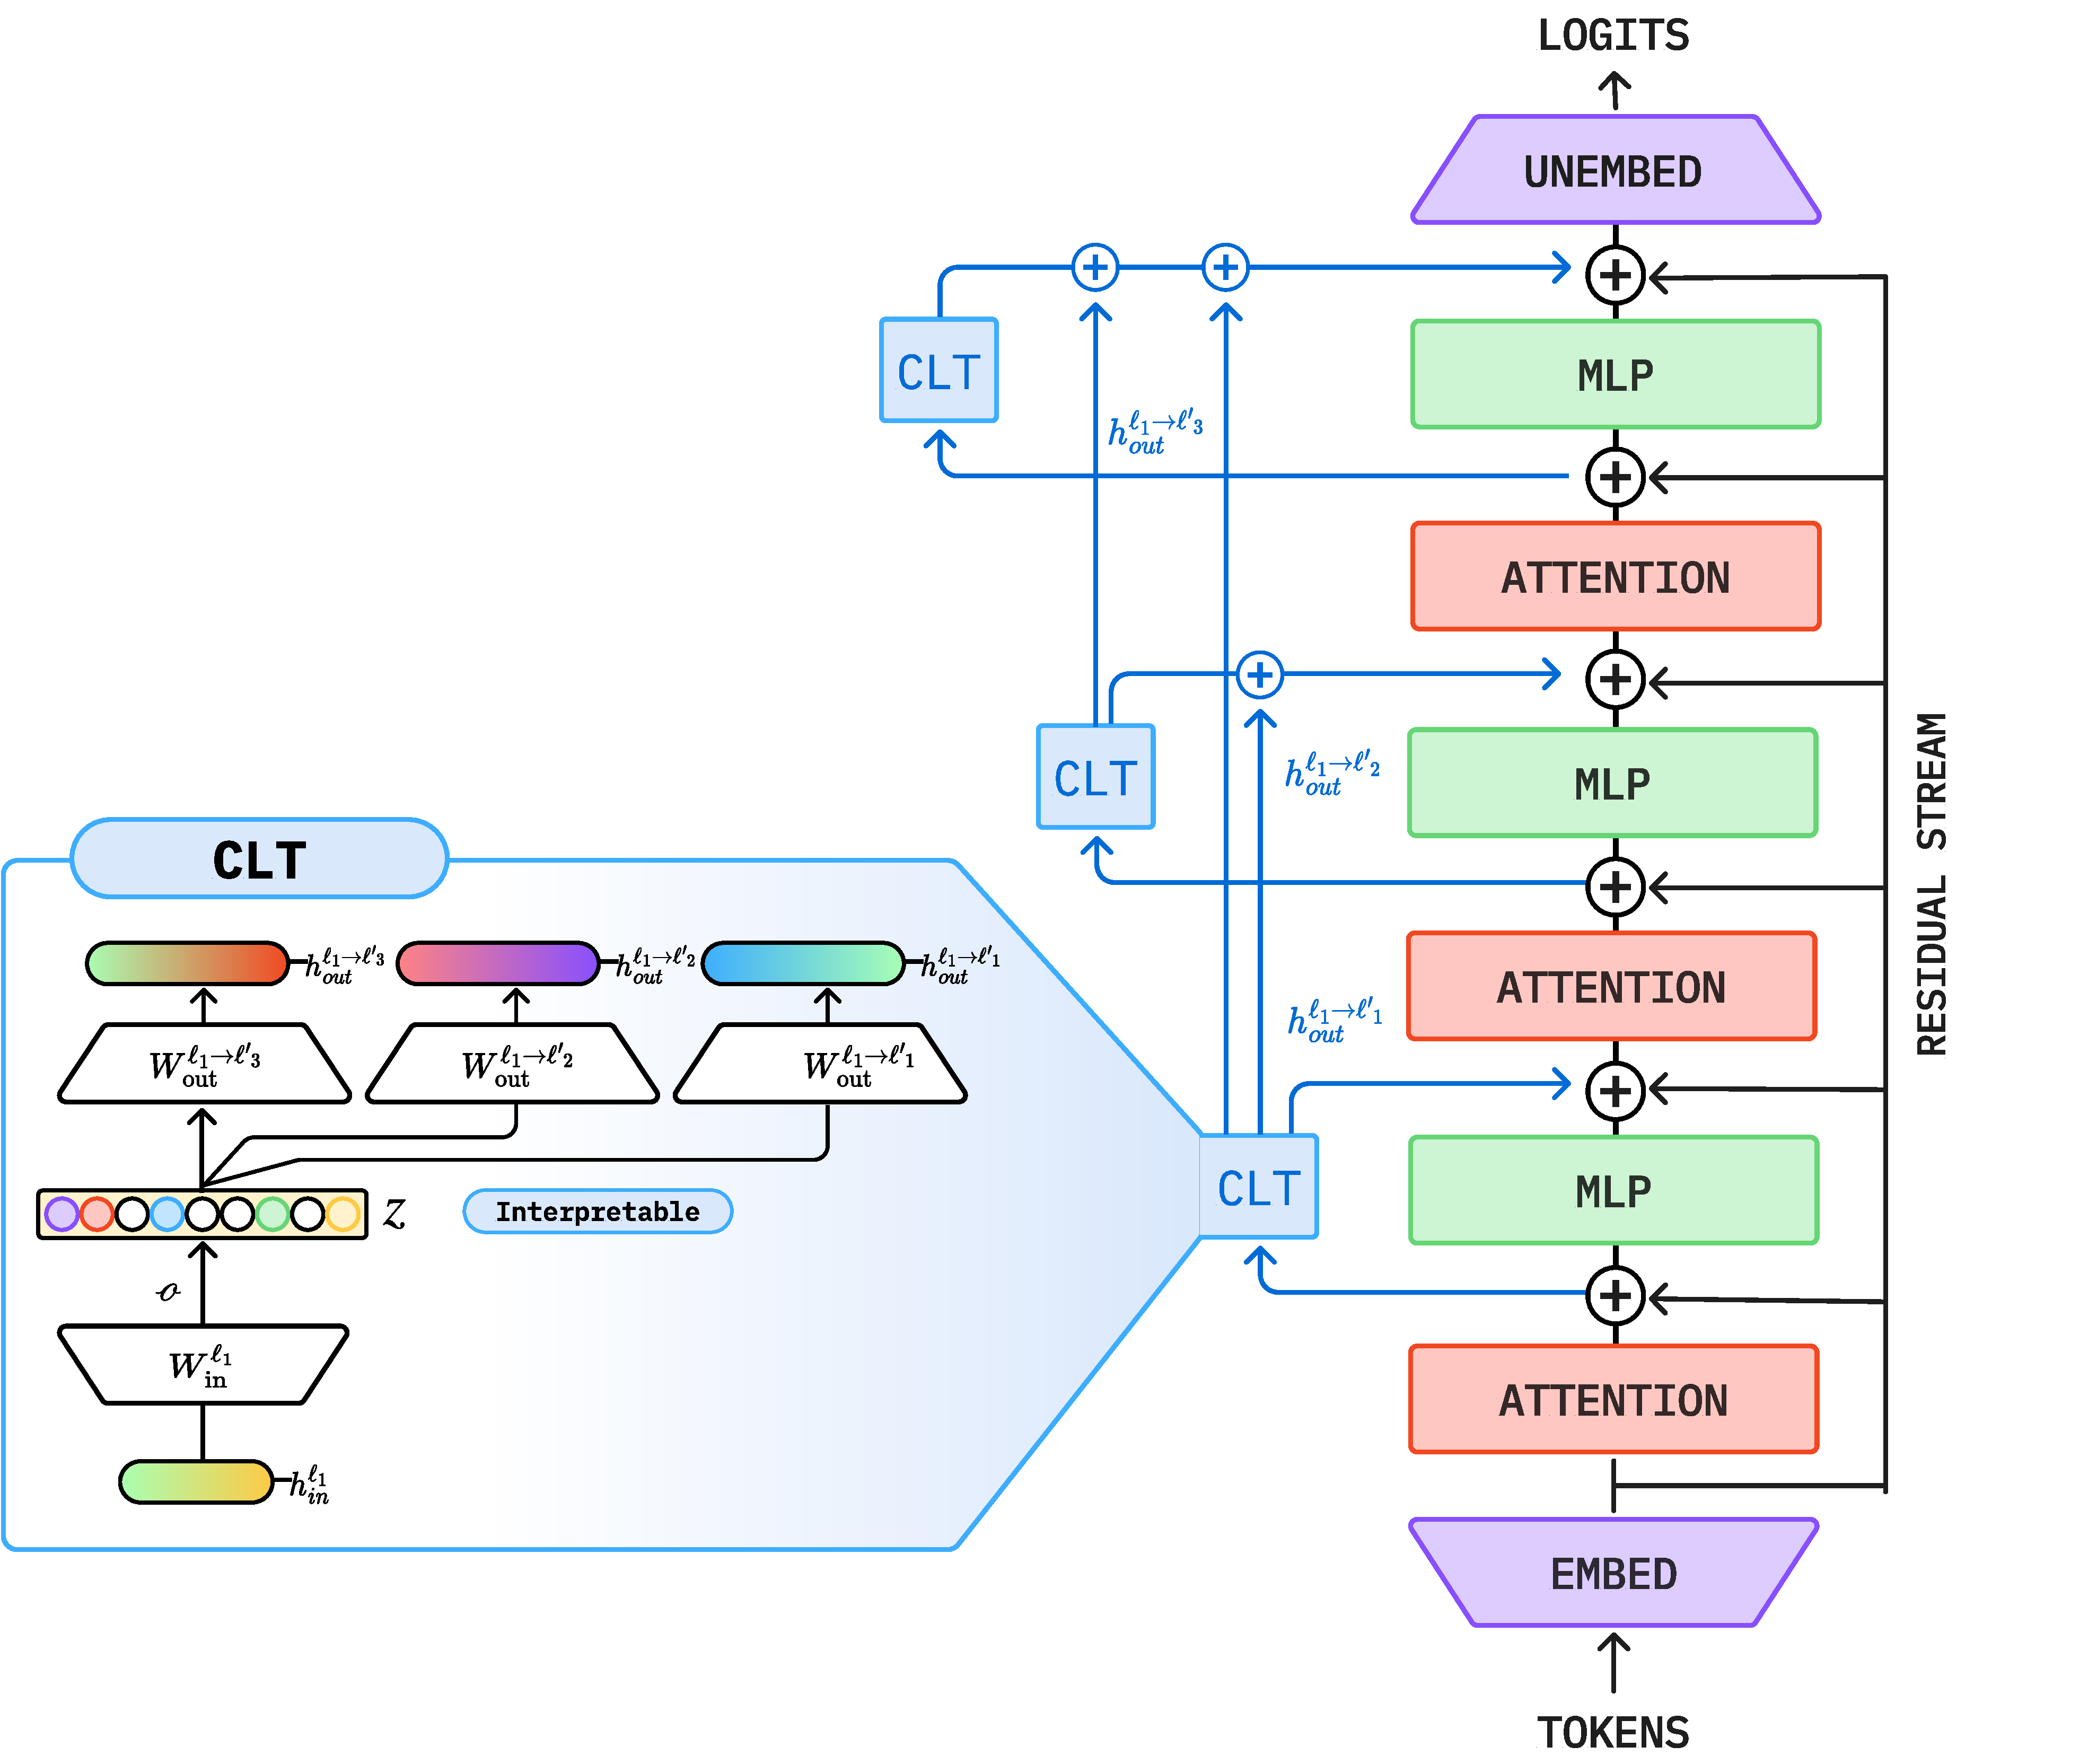
\includegraphics[width=\linewidth]{figs/6_CLT.pdf}
    \caption{Cross-layer transcoder.}
    \label{fig:clt}
  \end{subfigure}
  \caption{\textbf{Transcoders and CLTs.} Transcoders reconstruct the output of the MLP from its input in the same transformer layer. CLTs extend this by
  partially reconstructing the outputs of multiple subsequent layers from a
  single point in the residual stream.}
\end{figure}

\subsubsection{Cross-Layer Transcoders: Enabling Better Circuit Analysis}
\label{subsubsec:cross-layer-transcoder}

\begin{definitionbox}[Cross-Layer Transcoder (Figure~\ref{fig:clt})]
\emph{Cross-layer transcoders} (CLTs) are sparse feature decompositions spanning all layers of a neural network. At each layer $\ell$, sparse feature activations are read from the residual stream via
\[
z_{\ell}
=
\sigma_{\text{JumpReLU}}
\!\left(
W_{\text{in}}^\ell h_{\ell}^{\text{in}}
\right),
\]
where $z_\ell^j$ denotes the activation of feature $j$ at layer $\ell$.\\

Each feature can write to the MLP outputs of its own layer and all subsequent layers through layer-specific decoder vectors. The contribution from features read at layer $\ell$ to the MLP output at a subsequent layer $\ell'$ is
\[
\hat{h}_{\ell \to \ell'}^{\text{out}}
=
\sum_j
W_{\text{out},j}^{\ell \to \ell'} z_{\ell}^{j},
\]
where $W_{\text{out},j}^{\ell \to \ell'}$ is the decoder vector from feature $j$ at layer $\ell$ to the MLP output at layer $\ell'$. The reconstructed MLP output at layer $\ell'$ is then
\[
\hat{h}_{\ell'}^{\text{out}}
=
\sum_{\ell=1}^{\ell'}
\hat{h}_{\ell \to \ell'}^{\text{out}}
=
\sum_{\ell=1}^{\ell'}
\sum_j
W_{\text{out},j}^{\ell \to \ell'} z_{\ell}^{j},
\]
which approximates the original MLP output $h_{\ell'}^{\text{out}}$.
\end{definitionbox}

CLTs (Figure~\ref{fig:clt}) are trained jointly across all $L$ layers to minimise
\[
\mathcal{L}
=
\sum_{\ell'=1}^{L}
\left\|
\hat{h}_{\ell'}^{\text{out}}
-
h_{\ell'}^{\text{out}}
\right\|_2^2
+
\lambda
\sum_{\ell=1}^{L}
\sum_j
\tanh\!\left(
c\,
z_{\ell}^{j}
\sqrt{
\sum_{\ell'=\ell}^{L}
\left\|
W_{\text{out},j}^{\ell \to \ell'}
\right\|_2^2
}
\right),
\]
where $c$ is the sharpness hyperparameter~\citeem{ameisen2025circuit}.

\paragraph{Replacement Models and Attribution Graphs.}
A key insight is that CLTs enable the construction of a \emph{replacement model}---a version of the original model in which all MLP layers are replaced with their CLT reconstructions. Running this replacement model involves:
\begin{itemize}
    \item Computing CLT feature activations $z_{\ell}$ at each layer $\ell$
    \item Replacing MLP outputs $h^{\text{out}}_{\ell}$ with reconstructions $\hat{h}^{\text{out}}_{\ell}$ from features in layer $1$ through $\ell$
    \item Keeping attention layers unchanged
\end{itemize}

When analysing a specific prompt, the replacement model freezes the original model's attention patterns and normalisation statistics from its forward pass, then adds layer-specific error corrections. Under these conditions, the local replacement model can exactly match the original model's activations on that prompt while decomposing it into interpretable CLT features. However, when the model's activations are completely replaced by CLT reconstructions, the intervened model's top-1 predictions match the original model's on only about 50\% of prompts from the Pile dataset~\citeem{gao2020pile}. Notably, this experiment uses a relatively small, 18-layer transformer~\citeem{ameisen2025circuit}. Therefore, this figure should be interpreted with important caveats (see below).

\begin{warningbox}[Caveats on CLT Fidelity Claims]

CLTs have been claimed to possess high output fidelity given that they achieve high top-1 token agreement. However, this claim requires careful examination:\\

\paragraph{Conditions for reported fidelity:}
\begin{itemize}
    \item Results are reported primarily on toy or small models, whose generality to other model architectures (e.g., Llama, Qwen) and model sizes (e.g., 70B models) is underexplored.
    \item Fidelity was measured on short sequences in the CLT training data. Evaluation under distribution shift (e.g., out-of-domain tasks, adversarial inputs) is not adequate.
    \item The paper reports top-1 token agreement as the main result, while softer metrics (e.g., top-5 agreement, KL divergence) may show different patterns and insights.
\end{itemize}

\paragraph{Conditions for exact local matching:}
\begin{itemize}
    \item Attention patterns must be frozen from the original forward pass since the CLT does not compute or reconstruct attention computations.
    \item Layer normalisation statistics (means, variances) must be cached from the original model. The replacement model does not recompute these.
    \item Error correction terms are added per layer to compensate for reconstruction residuals. Without them, exact matching fails.
\end{itemize}

\paragraph{Factors affecting fidelity:}
\begin{itemize}
    \item \textit{Model scale}: Preliminary evidence suggests that reconstruction quality and feature interpretability improve with CLT model size. This may be because larger CLTs produce more structured, less entangled representations~\citeem{ameisen2025circuit}. However, systematic scaling studies are limited.
    \item \textit{Layer depth}: Early layers’ and late layers’ activations are usually input-specific and output-constrained, respectively. Middle layers have richer information derived from the input but have not yet converged to the output. As a result, middle layers often show higher reconstruction fidelity.
    \item \textit{Domain}: Fidelity on factual recall and syntactic tasks is higher than on complex reasoning or arithmetic tasks, where MLP computations may be more complex and cannot be approximated by sparse linear features.
\end{itemize}

These caveats do not invalidate CLTs as a tool for mechanistic analysis, but they do mean that fidelity should be verified on the target model and specific task before drawing strong conclusions from CLT-based circuit analysis.
\end{warningbox}

\paragraph{Why CLTs Enable Better Circuit Analysis.}
Unlike per-layer transcoders, CLTs reveal direct feature-to-feature interactions across layers: a feature in layer $\ell$ directly influences features in later layers through its contribution to their inputs. This simplifies circuit structure---features need not re-encode information at each layer. Additionally, replacing MLPs with CLT reconstructions makes the remaining computation \textit{approximately} linear (with frozen attention patterns and normalisation), enabling principled attribution: each feature's activation can be expressed as the sum of its input edges up to its activation threshold~\citeem{ameisen2025circuit}.

However, linearisation depends on several assumptions:
\begin{itemize}
    \item \textbf{Attention freezing:} By caching attention patterns, the replacement model treats attention as a fixed routing operation rather than a dynamic, input-dependent computation. This means CLT-based circuits describe model computation conditioned on \emph{given} attention patterns without analysing them.
    \item \textbf{Normalisation caching:} CLT analysis caches the input-dependent normalisation factors (e.g., LayerNorm denominators) from the original forward pass and reuses them during attribution instead of recomputing them after interventions. This removes a source of nonlinearity, but if an intervention would substantially change these normalisation factors in the original model, the cached computation no longer faithfully represents the intervened state.

    \item \textbf{Sparse linear approximation:} Dictionary learning methods assume MLP outputs or transformations are well approximated by sparse linear combinations of features. This assumption may fail when computations involve complex feature interactions or highly nonlinear transformations.
\end{itemize}

CLTs provide a powerful lens for circuit discovery when these assumptions hold. When they fail, CLT-based explanations may become unfaithful.

\paragraph{Computational Cost and Practical Considerations.}

\begin{figure}[th]
\centering
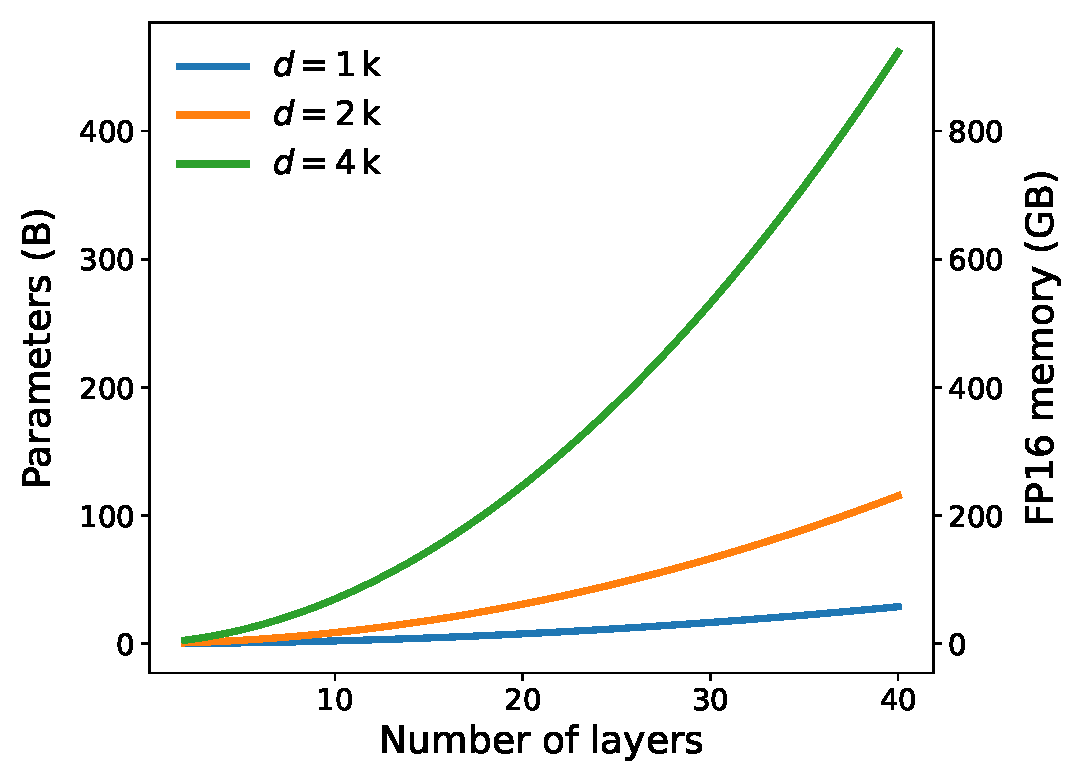
\includegraphics[width=0.7\linewidth]{figs/clt_size_vs_depth_e32_clean_v3.pdf}
    \caption{
    Parameter count (left) and FP16 memory requirements (right) of a full
    cross-layer transcoder as a function of model depth, for different residual
    stream dimensions and expansion factor $e=32$.
    }
\label{fig:clt-size-vs-depth}
\end{figure}

Let $d_{\text{sparse}} = ed$, where $e$ is the expansion factor. For a transformer with $L$ layers, a complete suite of CLTs contains $L$ encoders mapping
$
\mathbb{R}^d \rightarrow \mathbb{R}^{ed}
$
and $L(L+1)/2$ decoders mapping
$
\mathbb{R}^{ed} \rightarrow \mathbb{R}^d.
$
The resulting parameter count, with biases ignored, is therefore
\[
N_{\text{CLT}}(L,d,e)
=
\frac{e d^2}{2}\left(L^2 + 3L\right),
\]
which highlights the quadratic scaling with both model depth and hidden dimension, as illustrated in Figure~\ref{fig:clt-size-vs-depth}.

Training a suite of CLTs thus incurs a high upfront cost. For reference, training the CLT suite for Gemma-2-9B
required approximately 3{,}844 H100 GPU-hours at 50\% FLOPs efficiency~\citeem{ameisen2025circuit}. This cost is amortised over many circuit analyses on the trained CLT. The resulting interpretability gains (cross-layer features, lower interference, better attribution) justify the investment for systematic mechanistic analysis. 

For these reasons, current applications of CLTs remain limited: a ``greater-than'' mechanism
study~\citeem{merullo2025replicating}, an open-source
extension~\citeem{lindsey2025landscape}, and analysis of multilingual representations using CLTs~\citeem{harrasse2025tracing}. This scarcity of downstream use cases likely reflects the considerable challenges of training CLTs at scale and the complexity of using CLT-based circuit discovery in the wild.

\paragraph{Open Questions for CLT Research.}
Several important questions remain open:
\begin{itemize}
    \item How does CLT fidelity scale in large models? How can we better measure fidelity?
    \item Can CLTs be extended to model more nonlinearities such as attention patterns and normalisation, while maintaining their explanatory power?
    \item Can we develop evaluation protocols that reliably detect the potential unfaithfulness of CLT-based explanations?
    \item How sensitive are CLT circuits to experimental setups, such as the choice of training data?
\end{itemize}

\subsubsection{Crosscoders: Analysing Cross-Layer Features}

\begin{definitionbox}[Crosscoder (Figure~\ref{fig:crosscoders})]
A \emph{crosscoder} learns a shared sparse representation from activations across $L$ layers. It jointly encodes activations from all layers as
\[
z
=
\sigma_{\text{ReLU}}
\left(
\sum_{\ell=1}^{L}
W_{\text{in}}^\ell h_\ell
+
b_{\text{in}}
\right),
\]
where $z \in \mathbb{R}^{d_{\text{sparse}}}$ denotes the shared sparse feature activations and $W_{\text{in}}^\ell$ is the layer-$\ell$ encoder. Each layer is then reconstructed using a layer-specific decoder:
\[
\hat{h}_\ell
=
W_{\text{out}}^\ell z
+
b_{\text{out}}^\ell,
\qquad
\ell = 1,\ldots,L.
\]
Thus, a single latent feature can capture patterns that are shared across, persist through, or vary across multiple layers of the residual stream~\citeem{lindsey2024sparsecrosscoders}. Studies have also used crosscoders to discover shared features in activations from different models~(\citeestalp{ge2026evolution, bayazit-etal-2026-crosscoding}; \citeemalp{lindsey2024sparsecrosscoders, jiralerspong_cross-architecture_2025}), as detailed in Section~\ref{sec:model-diffing}.
\end{definitionbox}

\begin{figure}[tb]
  \centering
  \centering
    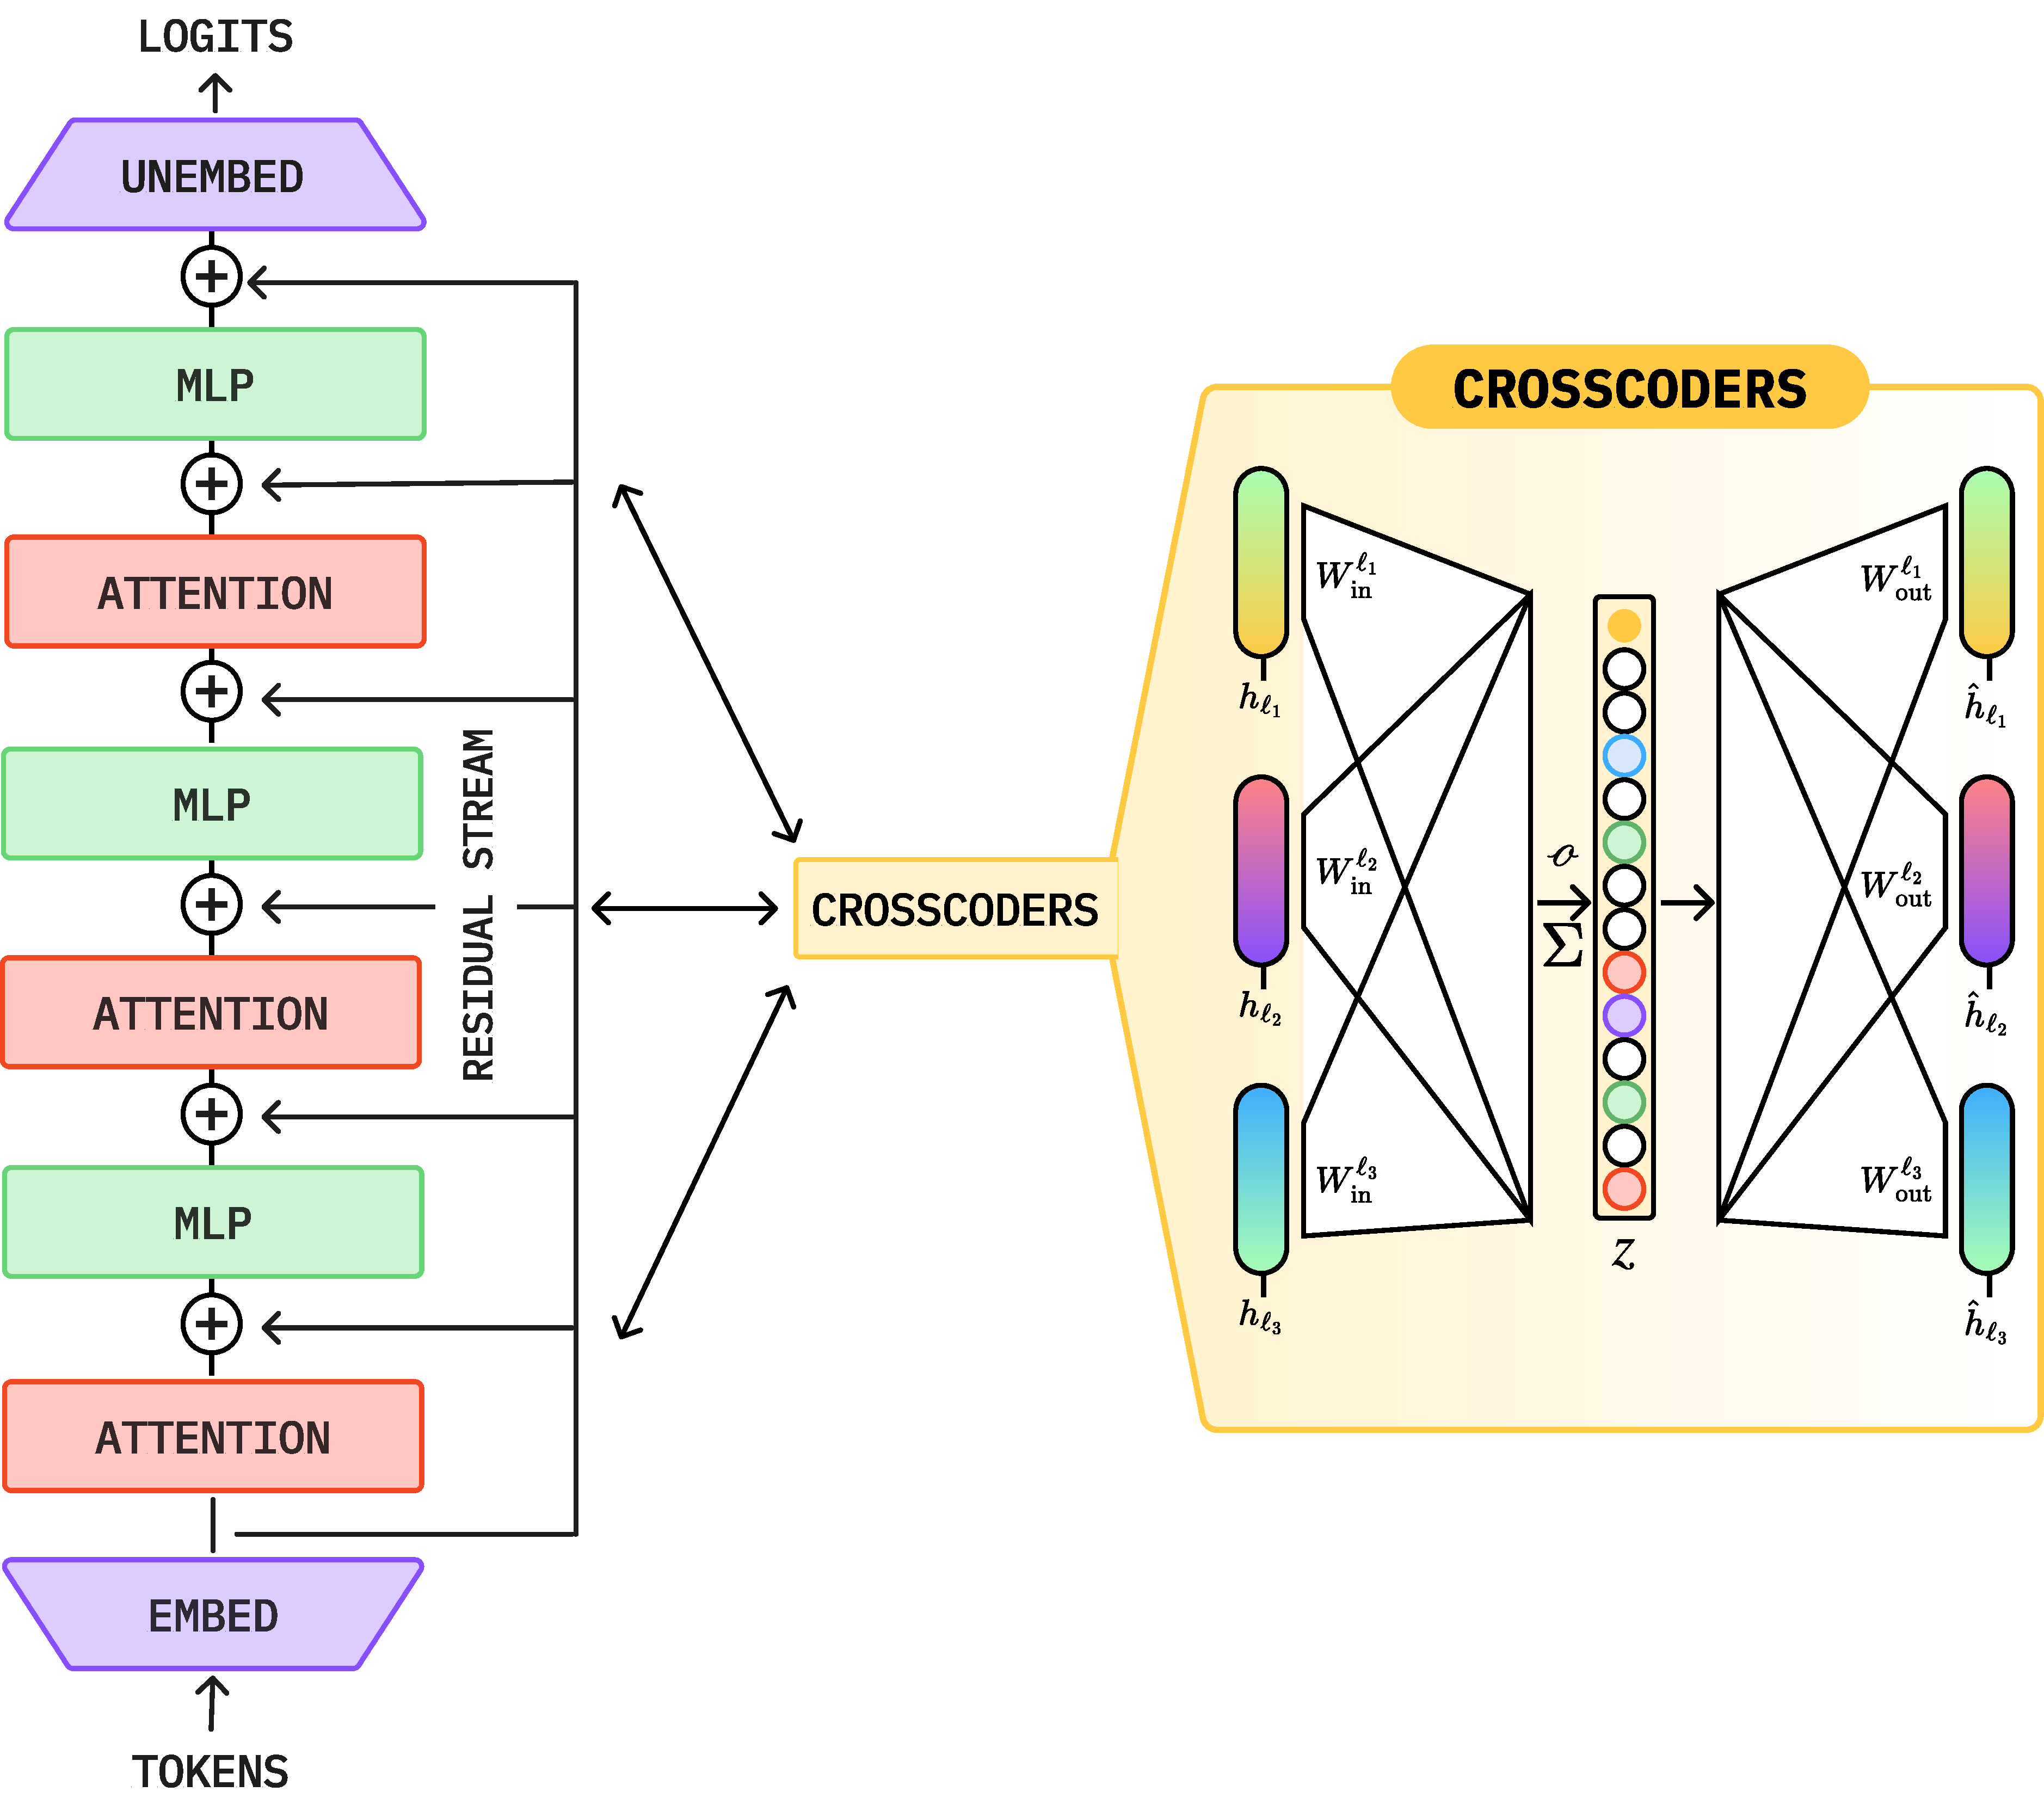
\includegraphics[width=0.7\linewidth]{figs/6_Crosscoders.pdf}
    \caption{\textbf{Crosscoder.} Crosscoders are trained to reconstruct the residual stream across multiple layers simultaneously.}
    \label{fig:crosscoders}
\end{figure}

A crosscoder is trained by minimising
\[
\mathcal{L}
=
\sum_{\ell=1}^{L}
\left\|
\hat{h}_\ell - h_\ell
\right\|_2^2
+
\lambda
\sum_j
\left(
\sum_{\ell=1}^{L}
\left\|
W_{\text{out},j}^{\ell}
\right\|_2
\right)
z^j,
\]
where $W_{\text{out},j}^{\ell}$ denotes the decoder vector of feature $j$ at layer $\ell$, and $\lambda$ controls the sparsity penalty.

\paragraph{Causal vs.\ Acausal Crosscoders.}
Crosscoders support two information flow patterns:
\begin{itemize}
    \item \textbf{Causal Crosscoders:} Read only from layers $\ell' \leq \ell$ at the current position. This respects the forward pass causality: earlier layers cannot read from later layers.
    \item \textbf{Acausal Crosscoders:} Read from any layer $\ell'$ regardless of depth ordering. Useful for understanding post-hoc feature relationships across the full model.
\end{itemize}

\paragraph{Applications to Circuit Analysis.}
By extracting cross-layer features, crosscoders help us understand how features propagate through the residual stream across layers, removing duplicate feature representations that complicate circuit analysis. This simplification allows features to ``jump'' across intervening identity operations, substantially reducing circuit complexity. More importantly, crosscoders reveal how input-relevant features transform as they flow through the network, distinguishing which features persist unchanged versus which are actively modified by downstream computation~\citeem{lindsey2024sparsecrosscoders}.

\subsection{Comparing SAEs, Transcoders, and Crosscoders}

Single-layer SAEs are efficient and locally interpretable but miss cross-layer feature evolution. Transcoders improve this by imitating MLP behaviour and revealing nonlinear transformations, though they require sequential analysis across depth. Cross-layer transcoders span multiple layers for global information flow but are extremely expensive. Crosscoders take a different approach, extracting shared features across layers simultaneously to resolve cross-layer superposition and simplify circuits without chaining predictions.


\subsection{Case Study: Induction Heads}
\label{subsec: induc head case study: feature extract}
Here, we examine induction heads~\citeem{olsson2022incontextlearninginductionheads}, a mechanism found in many modern language models, as a case study. We first describe their conditional-copying function and role in in-context learning, and then relate them to feature-extraction methods such as SAEs and CLTs, which reveal how this computation can be distributed across broader feature circuits.

\begin{definitionbox}[Induction Heads]
\label{def:induction-heads}

\emph{Induction heads}, first identified and analysed by
\citetem{elhage2021mathematical}, are attention heads that
implement a conditional copying rule over repeated subsequences. Let
$x=(x_1,\dots,x_T)$ be a token sequence, and consider positions $i<j<T$ such
that $x_i=x_j$. An attention head indexed $r$ (see Section~\ref{subsec:transformers} for an introduction to attention modules) is said to be an induction head when its
attention pattern assigns comparatively high attention weight from position
$j$ to position $i+1$ (i.e., high $A^r_{j,i+1}$) and its residual-stream update
\[
\Delta h^r
=
W_O^r V^r (A^r)^\top
\]
increases the model's logit for token $x_{i+1}$ when predicting the token at position $j+1$.\\

That is, induction heads implement the rule
\[
(x_i=x_j)
\;\Rightarrow\;
\hat{x}_{j+1}\approx x_{i+1}.
\]
They help enable in-context prediction by copying the continuation that followed an
earlier occurrence of the same token.

\end{definitionbox}

\begin{examplebox}[Induction in a Repeated Sequence]
Consider the sequence
\[
\texttt{A B C A B}
\]
where the model needs to predict the token after the second \texttt{B}. Observing the repeated prefix \texttt{A B}, an induction head attends from the second \texttt{B} to the position after the first \texttt{B} and contributes to the model’s prediction of \texttt{C}. This induction behaviour should generalise across tokens and positions.
\end{examplebox}


Induction heads were originally characterised as specific attention heads implementing this copying rule. However, subsequent work shows that we can understand the underlying computation more naturally at the level of distributed representations than at the level of isolated model components.

\begin{examplebox}[Induction Heads: Features Across Representations]

Feature extraction methods, such as SAEs, can decompose attention layer outputs into sparse, interpretable features that capture meaningful activation patterns beyond individual attention weights~\citeem{kissane2024interpretingattentionlayeroutputs}. Modern analyses suggest that induction heads are not isolated mechanisms but participate in distributed feature circuits, where multiple interacting features recur and compose across layers (\citeestalp{dunefsky2024transcodersinterpretablellmfeature, singh2024needsrightinductionhead}; \citeemalp{kissane2024interpretingattentionlayeroutputs, kamath2025tracing}).\\

SAEs trained on attention heads' activations reveal feature families of recurring patterns and contextual dependencies. Some of them align with behaviours originally attributed to induction heads~\citeem{kissane2024interpretingattentionlayeroutputs}. By analysing these features, we can understand how models maintain and manipulate information across tokens and contexts.\\

Cross-layer analyses, including crosscoders, suggest that certain features are represented consistently across layers rather than being recomputed at each layer~\citeem{lindsey2024sparsecrosscoders}. This perspective highlights that attention heads, including specialised ones such as induction heads, may be only part of broader, distributed feature representations.

\end{examplebox}

\subsection{Comparison with Alternative Feature Extraction Methods}

Besides SAEs, alternative techniques from signal processing and machine learning have also been adapted to extract features from neural networks. They make different modelling assumptions and therefore offer distinct trade-offs in interpretability, scalability, and robustness. Table~\ref{tab:decomposition-comparison} summarises the methods discussed in this section.

\begin{table}[tb]
\centering
\caption{Comparison of feature extraction methods.}
\label{tab:decomposition-comparison}
\renewcommand{\arraystretch}{1.3}
\begin{tabular}{>{\raggedright\arraybackslash}p{2.5cm} 
                >{\raggedright\arraybackslash}p{2.8cm} 
                >{\raggedright\arraybackslash}p{2.8cm} 
                >{\raggedright\arraybackslash}p{2.8cm} 
                >{\raggedright\arraybackslash}p{2.8cm}}
\toprule
\rowcolor{tableheader!80} \textcolor{white}{\textbf{Method}} & 
\textcolor{white}{\textbf{Assumption}} & 
\textcolor{white}{\textbf{Strengths}} & 
\textcolor{white}{\textbf{Weaknesses}} & 
\textcolor{white}{\textbf{Best Use Case}} \\
\midrule
\rowcolor{tablerow1} \textbf{SAE} & Sparse, linear features & Open-ended discovery; fast inference & Hyperparameter-sensitive; identifiability issues & Open-ended feature discovery \\
\rowcolor{tablerow2} \textbf{NMF} & Non-negative, additive parts & Parts-based interpretation; uniqueness guarantees & Requires non-negative data; limited sparsity & Naturally non-negative domains \\
\rowcolor{tablerow1} \textbf{PCA} & Variance aligns with features & Closed form; optimal low-rank reconstruction & Explains global variance and produces orthogonal features & Small-scale settings; as a baseline method \\
\rowcolor{tablerow2} \textbf{ICA} & Complete and independent sources & Theoretical guarantees when assumptions hold & Assumes independence; Gaussian blindness & When independence holds \\
\rowcolor{tablerow1} \textbf{Supervised methods} & Known concept labels & High performance on targeted concepts & Requires labels; no discovery & When certain concepts of interest are known \\
\rowcolor{tablerow2} \textbf{K-SVD} & Sparse, linear features & Explicitly solving the sparse-coding problem; no encoder bias & Slow inference; no learned encoder & Small, fixed sets of activations; as a baseline method \\
\bottomrule
\end{tabular}
\end{table}

\subsubsection{Non-Negative Matrix Factorisation}

Non-negative matrix factorisation (NMF; \citeestalp{lee1999learning}) decomposes a non-negative activation matrix $H \in \mathbb{R}^{d \times n}$ as $H \approx WA$, where both the feature dictionary $W \in \mathbb{R}^{d \times m}$ ($m$ is the preset number of features) and the coefficient matrix $A \in \mathbb{R}^{m \times n}$ are constrained to have non-negative elements. Because all components are non-negative, each feature contributes positively to the final representation, making it easier to interpret. Additionally, classical NMF’s optimisation process uses simple multiplicative update rules that preserve non-negativity. Moreover, under assumptions like \emph{separability} (each latent feature appears in at least one sufficiently ``pure'' example), NMF guarantees that the recovered decomposition is unique~\citeest{NIPS2003_1843e35d}.

However, classical NMF is not suitable for neural network activations because they can have negative elements, requiring additional preprocessing steps that may distort the activation-space structure. Moreover, NMF does not explicitly encourage feature sparsity, and scaling NMF to large dictionaries is computationally expensive. As a result, empirical work on extracting and analysing features in neural network activations has largely focused on Semi-NMF~\citeest{snmf}, which relaxes the non-negativity constraint on $W$. \citetest{shafran-etal-2026-constructing} showed that Semi-NMF can recover features competitive with SAEs on small-scale evaluations, but systematic comparisons at large scale remain limited. \citetem{yun-etal-2021-transformer} used a Semi-NMF-like approach to factorise BERT's contextualised hidden-state representations~\citeest{devlin2019bert}, allowing elements in $W$ to take both positive and negative values while constraining $A$ to be non-negative.



\subsubsection{Principal Component Analysis}
Principal Component Analysis (PCA; \citeestalp{pearson1901lines, hotelling1933analysis}) decomposes activations by finding an orthonormal basis of directions that maximise explained variance. Given a mean-centred activation matrix $H \in \mathbb{R}^{d \times n}$, where each column is an activation vector, PCA computes a low-rank approximation $H \approx U \Sigma V^\top$, where the columns of $U$ are the principal directions ordered by explained variance. PCA is fast, stable, and scalable. However, PCA imposes constraints and inductive biases that may misalign with neural network activations. Specifically, it identifies principal directions that maximise explained variance in the activation distribution, but much of the information of interest is region- or context-dependent and cannot be captured by variance alone. Moreover, PCA constrains the principal directions to be orthogonal, but in practice the underlying features correlate or partially overlap. Recent benchmarks~\citeest{wu2025axbench} reflect this misalignment: PCA underperformed most baselines, including SAEs, on both steering and concept-detection evaluations. While PCA can outperform SAEs in some localisation settings~\citeest{mueller2025mib}, it still generally lags behind simple supervised baselines.

\subsubsection{Independent Component Analysis}

Independent Component Analysis (ICA; \citeestalp{hyvarinen2000independent}) decomposes activations $H \in \mathbb{R}^{d \times n}$ as $H \approx WS$, where $n$ is the number of data points. Note that ICA may look similar to NMF at first glance. However, they were developed for different use cases and thus rely on different assumptions and optimisation procedures. In ICA, each column in $W \in \mathbb{R}^{d \times m}$ is a mixing vector, and $m$ is the number of different source signals; each row in $S \in \mathbb{R}^{m \times n}$ is a source signal (a signal has $n$ data points), with $m$ source signals in total. These signals are optimised to be independent of one another. Thus, if model activations are linear mixtures of statistically independent ``foundational features'', ICA can provably recover those features.

However, these assumptions may not hold for neural network activations. Specifically, classical ICA typically expects the completeness property (number of latent sources equals the dimensionality of the observed representation), and overcomplete decompositions (which are what we expect in activations) would require additional extensions~\citeest{lewicki2000learning}. Moreover, underlying features may not be statistically independent, which further limits the applicability of classical ICA. Although early studies applied it to analyse neural network activations, they did not find interpretability gains over SAEs~\citeest{cunningham2023sparse}. This may partly reflect the challenges discussed above.

More recently, however, \citetem{liu2026icalensinterpretinglanguage} showed that ICA can achieve performance comparable to that of SAEs, arguing that its previously reported underperformance may stem from limitations of classical ICA implementations poorly suited to the scale and statistical structure of neural network activations. These findings leave open whether ICA should be regarded primarily as a simple classical baseline or as an approach with underestimated, substantial headroom for further development.

\subsubsection{Supervised Feature Extraction Methods}
\label{subsubsec: supervised_extraction}

When the concepts of interest are known in advance, supervised methods can directly optimise representations aligned with those targets. Examples include distributed alignment search (DAS), which uses supervision to learn a change of basis that aligns representations with high-level causal variables~\citeest{das}; Supervised Multi-Dimensional Scaling (SMDS), which projects activations to preserve concept-level similarities~\citeest{smds}; and probes, which fit a concept direction in contrastive class-conditioned activations~\citeest{marks2024the}.

Notably, despite its simplicity, probing has outperformed SAEs in concept detection~\citeest{wu2025axbench}. It has also become a standard tool for identifying safety-relevant concepts in model representations, including refusal behaviour and implanted backdoors~(\citeestalp{arditi2024refusallanguagemodelsmediated}; \citeemalp{macdiarmid2024sleeperagentprobes}). We discuss probing in detail in Section~\ref{subsec:probing}. We put it under Section~\ref{sec:intermediate-computation} because we view its central methodological contributions and technical challenges as the readout of human-interpretable information---often expressed in natural language---from model activations, rather than the extraction of monosemantic features or causal variables.

When labelled data is available, supervised approaches often outperform SAEs on concept detection and steering tasks~(\citeestalp{huang-etal-2024-ravel, wu2025axbench}; \citeemalp{chaudhary2024evaluating}). They also avoid choosing dictionary sizes or sparsity penalties, since the concept set determines complexity. However, these methods require labelled data for each concept and cannot discover previously unknown features. Therefore, supervised methods suit settings where predefined, crisp concepts matter, whereas SAEs remain preferable for exploratory analysis.

\subsubsection{Dictionary Learning Baselines}
Classical dictionary learning methods provide useful baselines for evaluating SAEs. Techniques such as K-SVD alternate between sparse coding and dictionary updates and converge under certain conditions~\citeest{aharon2006k}. Comparative studies suggest that SAEs' primary advantage is fast inference because the encoder learns to decompose all activations, while potentially sacrificing optimal sparsity~\citeest{oneill2025compute}. As such, classical dictionary learning can still achieve superior dictionary quality in some cases and thus remains an important reference point for assessing the added value of SAEs.

\subsection{Interpretability-by-Design Methods for Intrinsic Interpretability}
\label{sec:architectural-interventions}

The methods surveyed thus far in this section aim to extract and analyse more monosemantic units from polysemantic model activations. They share a common premise: the model's original representations are too entangled to be directly interpretable, so interpretability is applied post hoc to recover simpler units of analysis. A parallel research programme, which we term \emph{Interpretability-by-Design Methods for Intrinsic Interpretability}, inverts this premise by asking whether deep neural models can instead be designed to be mechanistically interpretable by construction~(\citeestalp{pearce2025bilinear, park2025monet, oldfield2024multilinear, yang2025mixture, gao2025weight}; \citeemalp{adler2025towards, draye2025spartan, dooms2025compositionality}). This subsection extends the discussion of this research direction.

Next, we introduce five approaches for constructing models that are more interpretable by design. Three impose model sparsity constraints at different levels: feature-sparse training (Section~\ref{subsubsec: solu}), weight-sparse training (Section~\ref{subsubsec: weight sparse transformer}), and attention-sparse training (Section~\ref{subsubsec: spartan}). The remaining two approaches instead modify the computational primitives themselves, using more interpretable operators as units of construction and analysis (Sections~\ref{subsubsec: molt} and~\ref{subsubsec: kan}).

Interpretability should be understood as a spectrum rather than a binary property. At least in their current form, these techniques do not make model computation completely or immediately understandable. Instead, they make models easier to analyse and ensure the analysis pipeline preserves more information about the original computation than post-hoc approximations. Table~\ref{tab:architectural-methods} summarises these approaches and their trade-offs.

\subsubsection{Feature-Sparse Training}
\label{subsubsec: solu}
Softmax linear units (SoLU; \citeemalp{elhage2022solu}) are an earlier attempt at architectural intervention. SoLU is a specialised activation function that applies a softmax-based transformation across the layer's $d_{\mathrm{mlp}}$ neurons. Specifically, given the pre-activation vector
\[
u = W_1 h + b_1 \in \mathbb{R}^{d_{\mathrm{mlp}}},
\]
SoLU calculates the activation values as
\begin{equation}
    \sigma_{\text{SoLU}}(u)
    =
    u \odot \mathrm{softmax}(u).
\end{equation}
This softmax-based transformation induces competition among neurons. When one neuron receives a large pre-activation value, the softmax suppresses the others' values, analogous to lateral inhibition. This competition encourages certain neurons to specialise and dominate, increasing the prevalence of monosemantic neurons associated with human-interpretable concepts. 

However, it also reveals an undesirable phenomenon: although many secondary neurons’ activations are suppressed to low magnitudes, these neurons remain polysemantic, with many features compressed into them. Later layer normalisation~\citeem{ba2016layernormalization} can amplify them and recover the polysemanticity property~\citeem{elhage2022solu}. The ``smuggling'' by layer normalisation suggests that imposing local interpretability constraints may not eliminate neural networks’ incentive to compress information through superposition. This issue motivates global constraints across the neural network, such as weight-sparse training discussed below.

\subsubsection{Weight-Sparse Training}
\label{subsubsec: weight sparse transformer}
A weight-sparse transformer~\citeest{gao2025weight} treats weight sparsity as an explicit structural constraint that is progressively strengthened during training. \citetest{gao2025weight} optimise the standard cross-entropy objective along with an $L_0$ constraint on model weights after each optimisation step. Specifically, within each weight matrix, they retain only the largest-magnitude parameters and set the rest to zero. The $L_0$ constraint anneals from a dense initialisation to the desired sparsity level over training. The resulting transformer has most weight parameters exactly zero, making the remaining computational structure much easier to decompose into small, task-specific circuits.

Its interpretability gains can be substantial. Under highly sparse regimes (e.g., $<1\%$ active weights), neurons receive input from far fewer upstream neurons, and the model’s circuits for specific capabilities or behaviours become much sparser. Mean-ablation experiments further confirm that these circuits are
both necessary and sufficient for the capability or behaviour.

\citetest{gao2025weight} characterised the trade-off between model capability and interpretability induced by weight sparsity. Increasing sparsity generally makes the model easier to decompose into small, interpretable circuits. However, it also degrades task performance, producing a capability--interpretability Pareto frontier. Nonetheless, the authors found that increasing model size can shift this frontier outward. At comparable task performance, larger sparse models can have substantially smaller, more interpretable circuits than smaller models; at comparable interpretability, they can retain stronger capabilities. This suggests that scaling model size alongside structural sparsity may offer a path to more interpretable yet high-capability models. However, preserving interpretability beyond tens of millions of nonzero parameters remains challenging, and weight-sparse training currently requires substantially more compute than traditional training.

\begin{table}[tb]
\centering
\caption{Comparison of interpretability-by-design methods.}
\label{tab:architectural-methods}
\renewcommand{\arraystretch}{1.3}
\begin{tabular}{>{\raggedright\arraybackslash}p{2.8cm} 
                >{\raggedright\arraybackslash}p{3.2cm} 
                >{\raggedright\arraybackslash}p{4cm} 
                >{\raggedright\arraybackslash}p{4cm}}
\toprule
\rowcolor{tableheader!80} \textcolor{white}{\textbf{Method}} & 
\textcolor{white}{\textbf{Approach}} & 
\textcolor{white}{\textbf{Interpretability Gain}} & 
\textcolor{white}{\textbf{Primary Limitation}} \\
\midrule
\rowcolor{tablerow1} \textbf{Feature-Sparse Training (SoLU)} & Softmax-gated activation function & Increased neuron monosemanticity & Layer normalisation smuggling displaces superposition
\\
\rowcolor{tablerow2} \textbf{Weight-Sparse Training} & $L_0$ constraint on parameters & More monosemantic neurons and much smaller circuits & Training instability and scalability \\
\rowcolor{tablerow1} \textbf{Attention-Sparse Training} & $L_0$ regularisation on attention & Makes attention patterns interpretable & Requires fine-tuning on a trained language model \\

\rowcolor{tablerow2} \textbf{MOLT} & Sparse mixture of linear transforms & Reveals implemented operations directly & Complexity of matrix analysis \\
\rowcolor{tablerow1} \textbf{KANs} & Learnable splines on edges & Symbolic formula extraction & Scalability to LLMs is unproven \\
\bottomrule
\end{tabular}
\end{table}
\subsubsection{Attention-Sparse Training}
\label{subsubsec: spartan}
In transformers, attention patterns produced by an attention head are usually \emph{diffuse}, i.e., every token attends to every other token. Diffuse attention patterns are difficult to interpret and audit. Previous studies have therefore explored \emph{attention-sparse training}, which aims to sparsify attention patterns to make them more interpretable~(\citeestalp{lei2025spartan}; \citeemalp{draye2025spartan}). Specifically, \citetest{lei2025spartan} proposed \emph{SPARse TrANsformer World model} (SPARTAN), an object-centric world model trained with $L_0$ regularisation on attention patterns and a constrained optimisation objective to maintain cross-entropy performance equal to that of a dense counterpart. \citetem{draye2025spartan} further adapted this technique to fine-tune and sparsify a trained language model's attention patterns.

After training (either from scratch or via fine-tuning), each attention head attends only to specific tokens, and the model performance remains close to the original. This result suggests that many attention patterns may be redundant noise. In CLT-based circuit discovery (see Section~\ref{sec:circuit-replacement}), \citetem{draye2025spartan} showed that sparsified attention patterns reduce the number of mediating components involved in feature-to-feature attribution, making the resulting attribution graphs easier to analyse. 

\subsubsection{Modifications of Computational Primitives: MOLT}
\label{subsubsec: molt}

One alternative approach to learning interpretable structure is to reconsider what the computational primitives should be~(\citeestalp{oldfield2025towards, park2025monet}; \citeemalp{braun2025interpretability, bushnaq2025stochastic}). A recent example is the sparse mixture of linear transforms (MOLT), which represents a conceptual shift from feature extraction towards transformation extraction~\citeem{anthropic2025molt}.

Standard SAEs and transcoders primarily decompose model activations into features. However, many algorithmic tasks, such as arithmetic or geometric reasoning, are more naturally described by \emph{operations} such as ``add 3'' or ``rotate a vector''. In these tasks, we want to know how the model transforms one activation into another through components like weight matrices in MLP blocks. To achieve this, MOLT replaces the MLP with a sparse mixture of learned linear transformation matrices. The basic unit of analysis becomes transformations applied to model activations rather than features.

For example, in a modular arithmetic task, MOLT can represent the concept of addition with a learned rotation matrix, which relates more directly to the underlying algorithm than a collection of state-specific features. More broadly, approaches that represent computational operations explicitly, as MOLT does, may facilitate the development of interpretable representations for tasks governed by systematic operations. We view Kolmogorov--Arnold Networks (KANs) as an approach that embodies this idea, as discussed below.

\subsubsection{Kolmogorov--Arnold Networks}
\label{subsubsec: kan}

Kolmogorov--Arnold Networks (KANs) represent one of the most radical departures from standard neural network architectures~\citeest{liu2025kan}. In conventional neural networks, each neuron receives outputs from upstream neurons through incoming edges weighted by scalar parameters, sums these weighted inputs, and then applies a fixed nonlinear activation function (the whole process can be represented as matrix multiplication in components like MLP blocks and attention modules in Section~\ref{subsec:transformers}). Inspired by the Kolmogorov--Arnold representation theorem, KANs place learnable nonlinear functions, typically parameterised using B-splines, on edges rather than using fixed nonlinear activation functions at nodes.

Specifically, consider a single KAN node receiving an input vector
$v = (v_1, \dots, v_d) \in \mathbb{R}^d$ from the previous layer. Its output is
\[
y = \sum_{i=1}^{d} \psi_i(v_i), \qquad \psi_i(v_i) = \sum_{m} c_{i,m} B_m(v_i),
\]
where $B_m(\cdot)$ denotes the $m$-th basis function, such as a cubic B-spline basis,
and $c_{i,m}$ is a learnable scalar coefficient. In this formulation, the edge is not scalar multiplication but a learnable univariate function $\psi_i(\cdot)$, and a node simply sums the outputs of its incoming edges. Intuitively, KANs shift nonlinear transformations from nodes to edges, offering an alternative way to structure and interpret neural network computations.

This design gives KANs an explicitly compositional and thus more interpretable structure. As the nonlinearities are univariate and can be visualised directly on individual edges, researchers can use techniques like symbolic regression to approximate and inspect the learned analytical expressions, such as rediscovering known physical equations. Although KAN training is currently more computationally expensive than training standard MLPs and has not yet been convincingly demonstrated at the scale of large language models, this architectural innovation points to an ambitious direction towards interpretable neural networks in which parameters correspond to mathematically meaningful functions.

\paragraph{Summary.} This section introduced several classical methods for feature extraction and analysis, followed by approaches that aim to make models intrinsically interpretable. However, whether features are recovered post hoc or induced by design, they remain units of analysis rather than complete explanations of the model's mechanism, i.e., how these units interact and causally influence one another. Section~\ref{sec:circuit} therefore shifts from individual features to \emph{circuits}: computational graphs of interacting components that describe how the model implements its behaviours.
